\documentclass[a4paper, 12pt]{article}
\usepackage{style}
\usepackage{hyperref}

%colori per tablle tabu
\definecolor{tableHeader}{RGB}{254, 61, 0}
\definecolor{tableLineOne}{RGB}{245, 245, 245}
\definecolor{tableLineTwo}{RGB}{254, 204, 188}
%define header tabelle tabu
\newcommand{\tableHeaderStyle}{
    \rowfont[c]{\leavevmode\color{white}\bfseries}
    \rowcolor{tableHeader}
}

\title{Analisi dei requisiti}
\author{Cyber13}
\date{March 2019}

\begin{document}
	\begin{titlepage}
		\centering Università degli Studi di Padova
		\line(1,0){350}\\
		\vspace{1.2cm}
		\logo
		\vspace{1.0cm}
		\centering{\bfseries\LARGE ANALISI DEI REQUISITI \\}
		\vspace{0.5cm}
		\centering{\slshape\large Gruppo Cyber13 - Progetto P2PCS\\}
		\vspace{0.5cm}
		\centering{\bfseries Informazioni sul documento \\}
		\line(1,0){240}\\
		% compilare i campi per ogni documento
		\begin{tabular}{r|l}
			{\textbf{Versione}} 			& 1.0.0\\
			{\textbf{Data Redazione}} 	& 05/04/2019\\	% aggiornare la data
			{\textbf{Responsabili}} 	& Matteo Squeri\\ & Andrea Casagrande\\	% aggiornare la data
			{\textbf{Redazione}} 		& Daniel Mirel Bira \\ & Elena Pontecchiani\\  & Ilaria Rizzo\\
			{\textbf{Verifica}} 		& Daniel Mirel Bira \\	&  Andrea Casagrande \\ & Fabio Garavello\\ 
			{\textbf{Approvazione}} 	& Andrea Casagrande\\
			{\textbf{Uso}} 				& Esterno\\
			{\textbf{Destinatari}} & GaiaGo\\	& Cyber 13\\ & Prof. Tullio Vardanega\\ & Prof. Riccardo Cardin\\
			{\textbf{Mail di contatto}} 	& swe.cyber13@gmail.com\\
		\end{tabular}\\
	\end{titlepage}

	\newpage
		\subfile{DiarioModificheAdR.tex}
	\newpage
		\tableofcontents
        	\newpage
	    	\listoffigures
	    	\newpage
        	\section{Introduzione}
                \subsection{Scopo del documento}
Il presente documento ha lo scopo di presentare un'analisi completa di tutti i \citgl{requisiti} e i \citgl{casi d'uso} individuati dal team Cyber13 per lo sviluppo del progetto \citgl{P2PCS}. La seguente analisi è scaturita sulla base dello studio del capitolato d'appalto e di colloqui con l'azienda proponente \citgl{GaiaGo}.

\subsection{Scopo del prodotto}
Lo scopo del prodotto è di estendere un'applicazione per ambiente Android, già esistente per il \citgl{car sharing} condominiale, a livello \citgl{peer-to-peer}. Inoltre viene richiesto di integrare meccanismi di \citgl{Gamification}, al fine di rendere l'esperienza dell'utente all'interno dell'applicazione più gradevole.

\subsection{Glossario}
Onde evitare ambiguità o incomprensioni di natura lessicale, si allega il \G.
All'interno del documento saranno presenti parole di ambito specifico, uso raro che potrebbero creare incomprensioni. Per una maggiore leggibilità tali parole sono riconoscibili all'interno dei vari documenti in quanto scritte in corsivo e con un 'g' a pedice tra barre orizzontali (per esempio \citgl{Glossario})
\subsection{Riferimenti}
\subsubsection{Riferimenti normativi}
\begin{itemize}
    \item Norme di Progetto: \NdP
    
\end{itemize}
\subsubsection{Riferimenti informativi}
\begin{itemize}
    \item Presentazione del capitolato C5
    \\ \url{https://www.math.unipd.it/~tullio/IS-1/2018/Progetto/C5.pdf}
    \item Presentazione del concetto gamification
    \\ \url{https://www.math.unipd.it/~tullio/IS-1/2018/Progetto/P4.pdf}
    \item Lucidi didattici contenenti materiale didattico affrontato durante il corso di Ingegneria del Software:
        \begin{itemize}
            \item Materiale riguardante i diagrammi UML dei casi d'uso:
            \\ \url{https://www.math.unipd.it/~tullio/IS-1/2018/Dispense/E05b.pdf}
            \item Materiale riguardante il documento "Analisi dei Requisiti":
            \\ \url{https://www.math.unipd.it/~tullio/IS-1/2018/Dispense/L08.pdf}
        \end{itemize}
        
    
\end{itemize}


                \newpage
            \section{Descrizione generale}
                \subsection{Obiettivi del prodotto}
Il prodotto ha come obiettivo l'implementazione di un'applicazione mobile \citgl{Android} in grado di gestire un sistema di condivisione dell'auto "\citgl{peer-to-peer}" e che includa al suo interno meccaniche di gioco. 


\subsection{Funzionalità del prodotto}
Le funzionalità principali offerte dal prodotto sono le seguenti:
\begin{itemize}
    \item Permettere agli utenti, iscritti alla piattaforma e in possesso di un'auto, di mettere in condivisione la propria vettura ad altri utenti;
    \item Permettere agli utenti sprovvisti di vettura di prenotare un mezzo all'interno della piattaforma con il quale compiere un determinato itinerario;
    \item Tutte le ulteriori funzionalità hanno lo scopo di utilizzare meccaniche di \citgl{gamification} affinché l'utente sia motivato a utilizzare l'applicazione.
    
\end{itemize}
\subsection{Caratteristiche degli utenti}
Il prodotto non si rivolge a classi d'utenza appartenenti ad uno specifico ambito: l'utenza dell'applicazione sarà molto generica per età, interessi, ambito sociale e culturale. In particolare l'applicazione riconosce due classi di utenza, non mutuamente esclusive:
\begin{itemize}
    \item Coloro in possesso di un'auto inutilizzata  che condividono attraverso il sistema al fine di ottenere retribuzioni (monetarie o come bonus all'interno dell'applicazione);
    \item Coloro sprovvisti di una vettura e che necessitano di un mezzo per compiere un determinato itinerario.
\end{itemize}

\subsection{Piattaforme di esecuzione}
Il prodotto finale verrà sviluppato su diverse piattaforme d’esecuzione:
\begin{itemize}
    \item  Il \citgl{backend} che può essere sviluppato interamente dal gruppo o utilizzare la piattaforma \citgl{Movens} fornita dal Proponente;
    \item Il \citgl{frontend} deve essere sviluppato su un'applicazione Android già esistente ma non implementata fornita dal Proponente.
\end{itemize}

\subsection{Vincoli}
L'utente, per usufruire del servizio, dovrà possedere un telefono con sistema operativo Android e scaricare l'applicazione dal nome \citgl{GaiaGo}. Dopo aver fatto Registrazione/Login l'utente potrà usufruire dei servizi che l'applicazione fornisce. 

                \newpage
            \section{Casi d'uso}
                Dopo un accurato studio si è stipulata una lista di casi d'uso presentata qui di seguito. Ognuno dei quali è riportato come specificato nel documento \NdP, nel punto 2.2.3.1.4.
\subsection{Attori dei casi d'uso}
\subsubsection{Attori primari}
  \begin{enumerate}
      \item Utente non autenticato: utente il quale accede alla piattaforma sprovvisto di un account personale sulla piattaforma e/o che non esegue l'operazione di login;
      \item Utente autenticato: utente in possesso di un account personale sulla piattaforma e che ha eseguito con successo l'operazione di login.
  \end{enumerate}
  
 \subsubsection{Attori secondari}
 \begin{enumerate}
     \item Aws;
     \item Facebook.
 \end{enumerate}
    
    
\subsection{Elenco dei casi d'uso}
   \subsubsection{UC 1-Breve presentazione all'uso dell'applicazione}
  
   
    \begin{itemize}
        \item \textbf{Attori primari}: Utente non autenticato;
        \item \textbf{Scopo e descrizione}: L'utente visualizza una guida di introduzione che spiega brevemente le funzionalità che l'app possiede. Eventualmente l'utente se non interessato può decidere di interrompere la visualizzazione della guida; 
        \item \textbf{Scenario principale}: L'utente non autenticato, dopo aver aperto l'applicazione visualizza la guida introduttiva di presentazione;
        \item \textbf{Precondizione}: Il sistema è funzionante e l'utente sprovvisto di account che ha appena scaricato l'applicazione vi entra;
        \item \textbf{Postcondizione}: L’utente ha  avuto delle nozioni riguardanti le funzionalità dell'applicazione oppure ha deciso di saltare parte della guida introduttiva.
    \end{itemize}
    
  

        \subsubsection{UC 2-Registrazione}
        \begin{itemize}
        \item \textbf{Attori primari}: Utente non autenticato;
        \item \textbf{Attori secondari}: Aws;
        \item \textbf{Scopo e descrizione}: L'utente desidera creare il proprio profilo personale all'interno della piattaforma; 
        \item \textbf{Scenario principale}:
            \begin{itemize}
                \item L'utente non autenticato accede alla piattaforma;
                \item L'utente che desidera registrare il proprio account seleziona la funzionalità "Registrati";
                \item L'utente inserisce le credenziali richieste per creare un account;
                \item L'utente conferma la registrazione.
            \end{itemize}
        \item \textbf{Scenario secondario}: L'utente non intende proseguire con l'operazione di registrazione: interrompe l'inserimento dei dati e la registrazione non viene effettuata.
        
        
        
        
        \item \textbf{Precondizione}: L'utente non è riconosciuto nel sistema;
        \item \textbf{Postcondizione}: L'utente viene registrato all'interno del sistema.
        \end{itemize}
        
        
            \paragraph{UC 2.1-Inserimento nome}
                \begin{itemize}
                \item \textbf{Attori primari}: Utente non autenticato;
                
                \item \textbf{Scopo e descrizione}: L'utente compila il campo nome per effettuare la registrazione; 
                \item \textbf{Scenario principale}: 
                    \begin{itemize}
                        \item L'utente non autenticato si trova nella sezione apposita di registrazione;
                        \item L'utente compila il campo "Nome".
                    \end{itemize}
                \item \textbf{Precondizione}: Il sistema fornisce una schermata in cui è possibile inserire il proprio nome per il nuovo account;
                \item \textbf{Postcondizione}: L'utente ha compilato il campo "Nome".
                \end{itemize}
                
                
            \paragraph{UC 2.2-Inserimento cognome}
                \begin{itemize}
                \item \textbf{Attori primari}: Utente non autenticato;
                
                \item \textbf{Scopo e descrizione}: L'utente compila il campo cognome per effettuare la registrazione; 
                \item \textbf{Scenario principale}: 
                    \begin{itemize}
                        \item L'utente non autenticato si trova nella sezione apposita di registrazione;
                        \item L'utente compila il campo "Cognome".
                    \end{itemize}
                \item \textbf{Precondizione}: Il sistema fornisce una schermata in cui è possibile inserire il proprio cognome per il nuovo account;
                \item \textbf{Postcondizione}: L'utente ha compilato il campo "Cognome".
                \end{itemize}
                
                
                \paragraph{UC 2.3-Inserimento mail}
                \begin{itemize}
                \item \textbf{Attori primari}: Utente non autenticato;
                
                \item \textbf{Scopo e descrizione}: L'utente compila il campo mail per effettuare la registrazione; 
                \item \textbf{Scenario principale}: 
                    \begin{itemize}
                        \item L'utente non autenticato si trova nella sezione apposita di registrazione;
                        \item L'utente compila il campo "E-mail".
                    \end{itemize}
                \item \textbf{Estensioni}: La compilazione del campo può fallire per le seguenti motivazioni:
                    \begin{itemize}
                        \item Il formato della mail inserita non è valido (UC 2.12); 
                        \item La mail inserita è già associata ad un altro account sulla piattaforma (UC 2.9);
                    \end{itemize}
                \item \textbf{Precondizione}: Il sistema fornisce una schermata in cui è possibile inserire la propria               mail per il nuovo account;
                \item \textbf{Postcondizione}: L'utente ha compilato il campo "E-mail".
                \end{itemize}
                
                
                
                
                
                \paragraph{UC 2.4-Inserimento password}
                \begin{itemize}
                \item \textbf{Attori primari}: Utente non autenticato;
                
                \item \textbf{Scopo e descrizione}: L'utente compila il campo password per effettuare la registrazione. L’utente deve poter inserire una password segreta allo scopo di impedire l’accesso da parte di terzi al proprio account. L’inserimento deve impedire di leggere direttamente la password durante la digitazione. I caratteri devono essere sostituiti da un segnaposto; 
                \item \textbf{Scenario principale}: 
                    \begin{itemize}
                        \item L'utente non autenticato si trova nella sezione apposita di registrazione;
                        \item L'utente compila il campo "Password";
                    \end{itemize}
                \item \textbf{Estensioni}:  La compilazione del campo può fallire per la seguente motivazione:
                    \begin{itemize}
                        \item Il formato della password inserita non è valido (UC 2.11);
                    \end{itemize}
                \item \textbf{Precondizione}: Il sistema fornisce una schermata in cui è possibile inserire la propria password per il nuovo account;
                \item \textbf{Postcondizione}: L'utente ha compilato il campo "Password".
                \end{itemize}

                
                \paragraph{UC 2.5-Ripeti password}
                \begin{itemize}
                \item \textbf{Attori primari}: Utente non autenticato;
                
                \item \textbf{Scopo e descrizione}: L'utente compila il campo di conferma password per effettuare la registrazione; 
                \item \textbf{Scenario principale}: 
                    \begin{itemize}
                        \item L'utente non autenticato si trova nella sezione apposita di registrazione;
                        \item L'utente compila il campo "Conferma Password".
                    \end{itemize}
                \item \textbf{Estensioni}:  La compilazione del campo può fallire per la seguente motivazione:
                    \begin{itemize}
                        \item La ripetizione della password non coincide con la prima digitazione (UC 2.8);
                    \end{itemize}
                
                \item \textbf{Precondizione}: Il sistema fornisce una schermata in cui è possibile confermare la propria               password per il nuovo account;
                \item \textbf{Postcondizione}: L'utente ha compilato il campo "Conferma Password", all'interno del quale viene confermata la password già inserita nel campo "Password".
                \end{itemize}
                
                
                \paragraph{UC 2.6-Inserimento username}
                \begin{itemize}
                \item \textbf{Attori primari}: Utente non autenticato;
              
                \item \textbf{Scopo e descrizione}: L'utente compila il campo username per effettuare la registrazione; 
                \item \textbf{Scenario principale}: 
                    \begin{itemize}
                        \item L'utente non autenticato si trova nella sezione apposita di registrazione;
                        \item L'utente compila il campo "Username".
                    \end{itemize}
                \item \textbf{Estensioni}:  La compilazione del campo può fallire per la seguente motivazione:
                    \begin{itemize}
                     \item Username già esistente all'interno della piattaforma (UC 2.10);
                    \end{itemize}
                \item \textbf{Precondizione}: Il sistema fornisce una schermata in cui è possibile inserire il proprio               username per il nuovo account;
                \item \textbf{Postcondizione}: L'utente ha compilato il campo "Username".
                \end{itemize}
                
                
                \paragraph{UC 2.7-Conferma}
            \begin{itemize}
                \item \textbf{Attori primari}: : Utente non autenticato;
                
                \item \textbf{Scopo e descrizione}: L'utente conferma le operazioni precedentemente effettuate; 
                \item \textbf{Scenario principale}:
                    \begin{itemize}
                        \item L'utente si trova nella sezione dedicata alla registrazione;
                        \item L'utente conferma l'operazione cliccando il pulsante apposito.
                    \end{itemize}
                \item \textbf{Estensioni}: La registrazione può fallire a causa del seguente errore di compilazione da parte dell'utente:
                \begin{itemize}
                \item Esistono dei campi vuoti (UC 2.13).
                \end{itemize}
                \item \textbf{Precondizione}: L'utente si trova in una schermata in cui è possibile dare la conferma
                dei dati inseriti;
                \item \textbf{Postcondizione}:L’utente ha espresso di voler procedere con la conferma dell'operazione e quindi il sistema memorizza la decisione.
            \end{itemize}
                
        
        
        \paragraph{UC 2.8-Visualizzazione errore di ripetizione password fallita}
            \begin{itemize}
                \item \textbf{Attori primari}: Utente non autenticato;
                \item \textbf{Scopo e descrizione}: La procedura di registrazione ha riscontrato un errore in merito ai
                dati inseriti durante la procedura di registrazione. Nello specifico l'errore è dovuto al fatto che il contenuto dei campi "Password" e "Ripeti password" non coincidono. Il sistema avvisa l'utente in merito all'errore riscontrato.
                \item \textbf{Scenario principale}: 
                    \begin{itemize}
                        \item L'utente ha inserito le proprie credenziali e ha confermato di voler effettuare la registrazione;
                        \item I campi password e ripeti password non contengono lo stesso contenuto, pertanto scatenano un errore.
                    \end{itemize}
                \item \textbf{Precondizione}: L'utente ha inserito le proprie credenziali e ha confermato la registrazione. L'utente tenta di registrarsi inserendo password non coincidenti;
                 \item \textbf{Postcondizione}: Viene notificato all'utente che si è verificato un errore in merito
                alla procedura di registrazione. L'utente ora è consapevole del fatto che la ripetizione della password richiesta nel campo "Ripeti password" non coincide con la prima digitazione.
            \end{itemize}
        
        
        
         \paragraph{UC 2.9-Visualizzazione errore di mail già associata a un altro account}
            \begin{itemize}
                \item \textbf{Attori primari}: Utente non autenticato;
                \item \textbf{Scopo e descrizione}: La procedura di registrazione ha riscontrato un errore in merito ai
                dati inseriti. Nello specifico l'errore è dovuto al fatto che la mail inserita nel campo "Mail" è già associata ad un altro account della piattaforma.
                \item \textbf{Scenario principale}: 
                    \begin{itemize}
                        \item L'utente ha inserito la propria mail;
                        \item La mail inserita nel campo "E-mail" è già associata a un altro account della piattaforma, pertanto viene scatenato un errore.
                    \end{itemize}
                \item \textbf{Precondizione}: L'utente tenta di registrarsi inserendo una mail già associata a un altro account presente sulla piattaforma;
                 \item \textbf{Postcondizione}: Viene notificato all'utente che si è verificato un errore in merito
                alla procedura di registrazione. L'utente ora è consapevole del fatto che la mail scelta è già associata ad un altro account presente sulla piattaforma.
            \end{itemize}
            
            
            
            
            \paragraph{UC 2.10-Visualizzazione errore di username già associato a un altro account}
            \begin{itemize}
                \item \textbf{Attori primari}: Utente non autenticato;
                \item \textbf{Scopo e descrizione}: La procedura di registrazione ha riscontrato un errore in merito ai
                dati inseriti. Nello specifico l'errore è dovuto al fatto che lo username inserito nel campo "Username" è già associato a un altro account della piattaforma.
                \item \textbf{Scenario principale}: 
                    \begin{itemize}
                        \item L'utente ha inserito un proprio username;
                        \item Lo username inserito nel campo "Username" è già associato a un altro account della piattaforma, pertanto viene scatenato un errore.
                    \end{itemize}
                \item \textbf{Precondizione}:  L'utente tenta di registrarsi inserendo uno username già associato a un altro utente;
                 \item \textbf{Postcondizione}: Viene notificato all'utente che si è verificato un errore in merito
                alla procedura di registrazione. L'utente ora è consapevole del fatto che lo username scelto è già associato ad un altro account.
            \end{itemize}
        
        
        
        
         \paragraph{UC 2.11-Visualizzazione errore di formato password errato}
            \begin{itemize}
                \item \textbf{Attori primari}: Utente non autenticato;
               
                \item \textbf{Scopo e descrizione}: La procedura di registrazione ha riscontrato un errore in merito ai
                dati inseriti. Nello specifico l'errore è dovuto al fatto che il formato della password inserita nel campo "Password" è errato. 
                \item \textbf{Scenario principale}: 
                    \begin{itemize}
                        \item L'utente ha inserito le proprie credenziali e ha confermato di voler effettuare la registrazione;
                        \item Il formato della password inserita nel campo "Password" non è corretto, pertanto viene scatenato un errore.
                    \end{itemize}
                \item \textbf{Precondizione}: L'utente ha inserito le proprie credenziali. L'utente tenta di registrarsi inserendo un formato per la password non consentito.
                 \item \textbf{Postcondizione}: Viene notificato all'utente che si è verificato un errore in merito
                alla procedura di registrazione. L'utente ora è consapevole del fatto che il formato della password scelta non è consentito.
            \end{itemize}
            
            
            
            \paragraph{UC 2.12-Visualizzazione errore di formato mail errato}
            \begin{itemize}
                \item \textbf{Attori primari}: Utente non autenticato;
                
                \item \textbf{Scopo e descrizione}: La procedura di registrazione ha riscontrato un errore in merito ai
                dati inseriti. Nello specifico l'errore è dovuto al fatto che il formato della mail inserita nel campo "E-mail" è errato.
                   
                \item \textbf{Scenario principale}: 
                    \begin{itemize}
                        \item L'utente ha inserito le proprie credenziali;
                        \item Il formato della mail inserita nel campo "E-mail" non è corretto, pertanto viene scatenato un errore.
                    \end{itemize}
                \item \textbf{Precondizione}:  L'utente tenta di registrarsi inserendo un formato per la mail non consentito.
                 \item \textbf{Postcondizione}: Viene notificato all'utente che si è verificato un errore in merito
                alla procedura di registrazione. L'utente ora è consapevole del fatto che il formato della mail scelta non è consentito.
            \end{itemize}
        
        
        
         
            \paragraph{UC 2.13-Visualizzazione errore di campi di compilazione vuoti}
            \begin{itemize}
                \item \textbf{Attori primari}: Utente non autenticato;
                
                \item \textbf{Scopo e descrizione}: La procedura di registrazione ha riscontrato un errore in merito ai
                dati inseriti. Nello specifico l'errore è dovuto al fatto che esiste almeno un campo di compilazione lasciato vuoto.
                  
                \item \textbf{Scenario principale}: 
                    \begin{itemize}
                        \item L'utente ha inserito le proprie credenziali e ha confermato di voler effettuare la registrazione;
                        \item L'utente non ha compilato uno o più campi.
                    \end{itemize}
                \item \textbf{Precondizione}: L'utente ha inserito le proprie credenziali e ha confermato la registrazione. L'utente tenta di registrarsi non compilando tutti i campi.
                 \item \textbf{Postcondizione}: Viene notificato all'utente che si è verificato un errore in merito
                alla procedura di registrazione. L'utente ora è consapevole del fatto che deve compilare tutti i campi per effettuare la registrazione.
            \end{itemize}
        
        \begin{figure}[h!]
           \begin{center}
           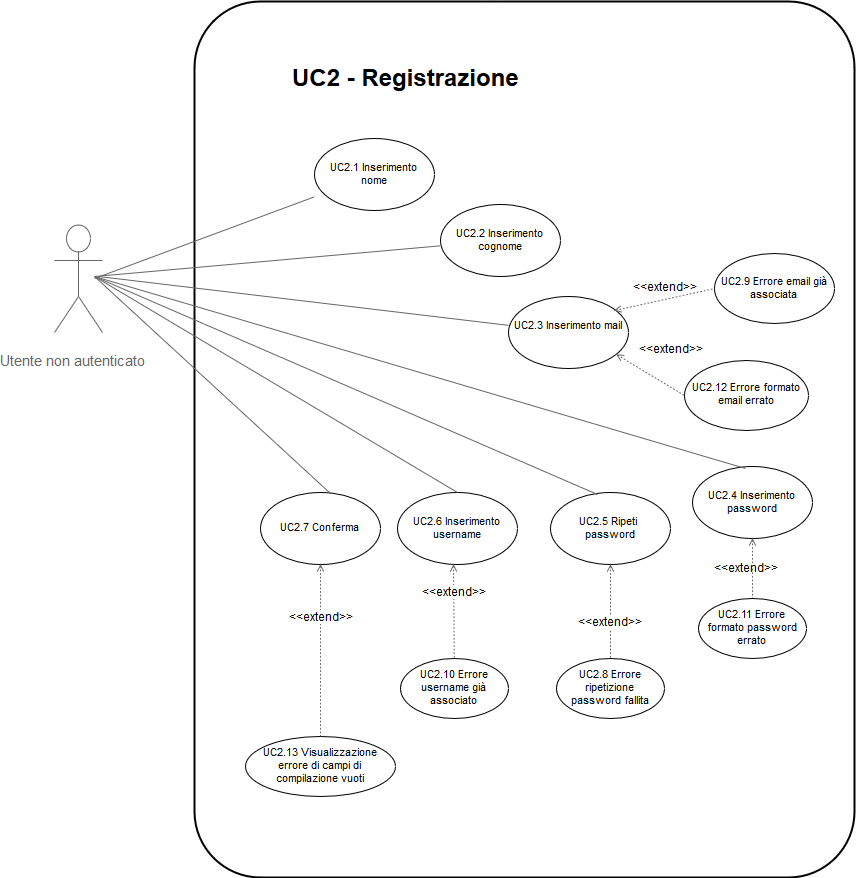
\includegraphics[scale=0.50]{immagini/2.png}
           \caption{Diagramma UC2 - Registrazione}
           \end{center}
        \end{figure}

 
 
        
      \subsubsection{UC 3-Login}
        \begin{itemize}
        \item \textbf{Attori primari}: Utente non autenticato.
        \item \textbf{Attori secondari}: Aws.
        \item \textbf{Scopo e descrizione}: L'utente richiede il login al sistema per accedere al proprio account.
        \item \textbf{Scenario principale}:
            \begin{itemize}
                \item L'utente non autenticato accede alla piattaforma;
                \item L'utente che desidera accedere al proprio account seleziona la funzionalità "Login";
                \item L'utente digita le credenziali di accesso relative al proprio account;
                \item L'utente conferma il login.
            \end{itemize}
         \item \textbf{Scenario secondario}: L'utente non desidera procedere con la conferma del login. Di conseguenza viene mostrata la schermata principale del sistema.
         
        \item \textbf{Precondizione}: L'utente non è riconosciuto nel sistema;
        \item \textbf{Postcondizione}: L'utente viene riconosciuto dal sistema.
        \end{itemize}

   
        \paragraph{UC 3.1-Inserimento username}
            \begin{itemize}
                \item \textbf{Attori primari}: Utente non autenticato;
                
                \item \textbf{Scopo e descrizione}: L'utente inserisce il proprio username per effettuare la login; 
                \item \textbf{Scenario principale}: 
                    \begin{itemize}
                        \item L'utente si trova nella sezione dedicata al login;
                        \item L'utente inserisce il proprio username.
                    \end{itemize}
                \item \textbf{Precondizione}: L'utente si trova in una schermata in cui è possibile inserire il proprio username;
             \item \textbf{Postcondizione}:L'utente ha inserito il proprio username.
           \end{itemize}
        
        \paragraph{UC 3.2-Inserimento password}
            \begin{itemize}
                \item \textbf{Attori primari}: Utente non autenticato;
                
                \item \textbf{Scopo e descrizione}: L'utente inserisce la propria password per effettuare la login. Durante l’inserimento non deve essere possibile leggere la password. Sarà possibile visualizzare
                dei segnaposto per indicare che è stato inserito un carattere della password; 
                \item \textbf{Scenario principale}: 
                    \begin{itemize}
                        \item L'utente si trova nella sezione dedicata al login;
                        \item L'utente inserisce la propria password.
                    \end{itemize}
                \item \textbf{Precondizione}: L'utente si trova in una schermata in cui è possibile inserire la propria password;
             \item \textbf{Postcondizione}:L'utente ha inserito la propria password.
           \end{itemize}
           
        \paragraph{UC 3.3-Conferma login}
            \begin{itemize}
                \item \textbf{Attori primari}: : Utente non autenticato;
                \item \textbf{Scopo e descrizione}: L'utente conferma i dati inseriti precedentemente per effettuare il login; 
                \item \textbf{Scenario principale}:
                    \begin{itemize}
                        \item L'utente si trova nella sezione dedicata al login;
                        \item L'utente conferma l'operazione di login cliccando il pulsante apposito.
                    \end{itemize}
                \item \textbf{Estensioni}: Visualizzazione errore nel caso di autenticazione fallita (UC 3.4), dovuta all'inserimento di credenziali errate;
                \item \textbf{Precondizione}:L'utente si trova in una schermata in cui è possibile dare la conferma dei dati inseriti;
                \item \textbf{Postcondizione}:L’utente ha espresso di voler procedere con la conferma e quindi con il login al sistema.
            \end{itemize}
        
        
        \paragraph{UC 3.4-Autenticazione fallita}
            \begin{itemize}
                \item \textbf{Attori primari}: Utente non autenticato;
                
                \item \textbf{Scopo e descrizione}: La procedura di autenticazione ha riscontrato un errore in merito ai
                dati inseriti durante la procedura di login.  
                   
                \item \textbf{Scenario principale}: 
                    \begin{itemize}
                        \item L'utente ha inserito le proprie credenziali e ha confermato il login;
                        \item Le credenziali inserite dall'utente non sono corrette, pertanto scatenano un errore di autenticazione.
                    \end{itemize}
                \item \textbf{Precondizione}: L'utente ha inserito le proprie credenziali e ha confermato il login;
                 \item \textbf{Postcondizione}: Viene notificato all'utente che si è verificato un errore in merito
                alla procedura di autenticazione. Deve essere indicato specificatamente che tipo di errore si è presentato.
            \end{itemize}
   \newpage
   
   \begin{figure}[h!]
           \begin{center}
           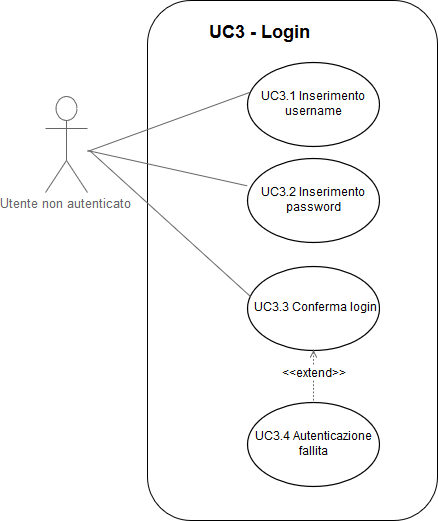
\includegraphics[scale=0.50]{immagini/3.png}
           \caption{Diagramma UC3 - Login}
           \end{center}
  \end{figure}   
          
       
        
     \subsubsection{UC 4-Logout}
        \begin{itemize}
            \item  \textbf{Attori primari}: Utente autenticato;
            \item \textbf{Scopo e descrizione}: L'utente che desidera effettuare il logout clicca su un apposita sezione e dà conferma.
            \item \textbf{Scenario principale}: L'utente precedentemente autenticato richiede il logout dal profilo personale interno all'applicazione;
            \item \textbf{Precondizione}: L'utente è autenticato e il sistema mette a sua disposizione una sezione apposita al logout;
            \item \textbf{Postcondizione}: Il sistema ha elaborato la richiesta di logout dell'utente chiudendo la sua sessione.
        \end{itemize}    
        
        
    \subsubsection{UC 5-Inserimento/modifica dei dati opzionali relativi all'account}  
      \begin{itemize}
        \item \textbf{Attori primari}: Utente autenticato;
        \item \textbf{Attori secondari}: Aws, Facebook;
        \item \textbf{Scopo e descrizione}: L'utente che ha precedentemente creato un profilo inserendo le informazioni obbligatorie desidera arricchire il suo profilo, inserendo per la prima volta o modificando le informazioni esistenti, con informazioni aggiuntive.
        \item \textbf{Scenario principale}:
            \begin{itemize}
                \item L'utente è autenticato con il proprio profilo all'interno del sistema;
                \item L'utente desidera arricchire il profilo inserendo o modificando i dati opzionali a esso associato, pertanto si porta nell'apposita sezione.
            \end{itemize}
        \item \textbf{Scenario secondario}: L'utente non desidera procedere con l'inserimento o la modifica dei dati opzionali;
        \item \textbf{Precondizione}: L'utente autenticato si trova nella propria area personale, nella sezione apposita per l'inserimento o la modifica dei dati opzionali del proprio profilo;
        \item \textbf{Postcondizione}: L'utente ha inserito o modificato i dati opzionali associati al proprio profilo.
        \end{itemize}


        
        \subsubsection{UC 6-Modifica dei dati anagrafici obbligatori del profilo utente}
        \begin{itemize}
        \item \textbf{Attori primari}: Utente autenticato;
        \item \textbf{Attori secondari}: Aws;
        \item \textbf{Scopo e descrizione}: L'utente autenticato è in grado di eseguire operazioni di modifica sui dati personali, precedentemente inseriti in fase di registrazione, o di eliminare il proprio account. I dati modificabili sono quindi:
            \begin{itemize}
                \item Nome;
                \item Cognome;
                \item Username;
                \item E-mail;
                \item Password.
            \end{itemize}
        \item \textbf{Scenario principale}:
            \begin{itemize}
                \item L'utente autenticato accede alla piattaforma;
                \item L'utente che desidera apportare modifiche al proprio account seleziona la specifica sezione per le modifiche all'account;
                \item L'utente modifica i propri dati secondo esigenze;
                \item L'utente conferma le modifiche apportate.
            \end{itemize}
        \item \textbf{Scenario secondario}: L'utente interrompe l'inserimento delle modifiche sui dati e le modifiche non vengono memorizzate dal sistema.
         \textbf{Precondizione}: L'utente autenticato ha scelto di apportare modifiche al proprio account;
        \item \textbf{Postcondizione}: Il sistema ha memorizzato le modifiche desiderate e permesse che l’utente ha apportato al proprio profilo.
        \end{itemize}
        
         \paragraph{UC 6.1-Modifica password}
            \begin{itemize}
                \item \textbf{Attori primari}: Utente autenticato;
               
                \item \textbf{Scopo e descrizione}: L'utente desidera modificare la propria password; 
                \item \textbf{Scenario principale}:
                    \begin{itemize}
                        \item L'utente si trova nella sezione dedicata alla modifica dei dati relativi all'account utente;
                        \item L'utente modifica la password relativa all'account.
                    \end{itemize}
                \item \textbf{Scenario secondario}: L'utente non desidera continuare con la modifica della password e termina l'inserimento. Il sistema non memorizza le modifiche apportate;
                 \item \textbf{Inclusioni}: 
                    \begin{itemize}
                        \item L'utente per poter memorizzare la nuova password deve inserire la password precedente (UC 6.1.1);
                        \item  L'utente per poter memorizzare la nuova password deve ripetere la password all'interno del campo "Ripeti password" (UC 2.5);
                    \end{itemize}
                \item \textbf{Estensioni}:
                    \begin{itemize}
                        \item La nuova password inserita è uguale a quella precedente (UC 6.1.2);
                        \item La conferma della nuova password inserita non coincide con la prima digitata (UC 2.8);
                        \item Il formato della nuova password inserita non è corretto (UC 2.11).
                    \end{itemize}
               
                \item \textbf{Precondizione}: L'utente si trova in una schermata in cui è possibile modificare la password associata al proprio profilo;
                \item \textbf{Postcondizione}:L’utente ha espresso di voler procedere con la conferma e quindi
                con la modifica della password associata al suo profilo.
            \end{itemize}
        
            \subparagraph{UC 6.1.1-Inserisci vecchia password}
                \begin{itemize}
                \item \textbf{Attori primari}: Utente autenticato;
               
                \item \textbf{Scopo e descrizione}: L'utente deve inserire la vecchia password per poterne inserire una nuova;
                \item \textbf{Scenario principale}:
                    \begin{itemize}
                        \item L'utente si trova nella sezione dedicata alla modifica dei dati personali relativi all'account utente;
                        \item L'utente inserisce la password antecedente relativa all'account per poterla aggiornare.
                    \end{itemize}
                \item \textbf{Precondizione}: L'utente si trova in una schermata in cui è possibile modificare i dati utente relativi all'account, nello specifico la password associata all'account;
                \item \textbf{Postcondizione}: L’utente ha inserito la vecchia password correttamente al fine di aggiornarla.
            \end{itemize}
        
        
         \subparagraph{UC 6.1.2-La nuova password coincide con quella precedente}
             \begin{itemize}
                \item \textbf{Attori primari}: Utente autenticato;
               
                \item \textbf{Scopo e descrizione}: L'utente deve inserire la vecchia password per poterne inserire una nuova, ma si verifica un errore dal momento che la nuova password inserita coincide con quella precedente.
                \item \textbf{Scenario principale}:
                    \begin{itemize}
                        \item L'utente si trova nella sezione dedicata alla modifica dei dati personali relativi all'account utente, nello specifico sta modificando la password associata al proprio account;
                        \item L'utente inserisce una nuova password uguale a quella precedente.
                    \end{itemize}
                \item \textbf{Precondizione}: L'utente si trova in una schermata in cui è possibile modificare i dati utente relativi all'account, nello specifico la password associata all'account;
                \item \textbf{Postcondizione}:L’utente non ha modificato la propria password poiché ha inserito una nuova password che coincide con quella vecchia: il sistema non registra le modifiche.
            \end{itemize}
        
        
        \paragraph{UC 6.2-Modifica mail}
            \begin{itemize}
                \item \textbf{Attori primari}: Utente autenticato;
               
                \item \textbf{Scopo e descrizione}: L'utente desidera modificare la mail associata all'account; 
                \item \textbf{Scenario principale}:
                    \begin{itemize}
                        \item L'utente si trova nella sezione dedicata alla modifica dei dati relativi all'account utente;
                        \item L'utente modifica la mail relativa all'account.
                    \end{itemize}
                \item \textbf{Estensioni}:
                    \begin{itemize}
                        \item La nuova mail è già associata a un profilo esistente (UC 2.9).
                        \item Il formato della nuova mail non è valido(UC 2.12).
                      \end{itemize}
                \item \textbf{Precondizione}: L'utente si trova in una schermata in cui è possibile modificare la propria mail;
                \item \textbf{Postcondizione}:L’utente ha espresso di voler procedere con la conferma e quindi
                con la modifica della propria mail.
            \end{itemize}
        
        \paragraph{UC 6.3-Modifica Nome}
            \begin{itemize}
                \item \textbf{Attori primari}: Utente autenticato;
                
                \item \textbf{Scopo e descrizione}: L'utente desidera modificare il nome associato al proprio account; 
                \item \textbf{Scenario principale}:
                    \begin{itemize}
                        \item L'utente si trova nella sezione dedicata alla modifica dei dati relativi al proprio account;
                        \item L'utente modifica il nome relativo all'account.
                    \end{itemize}
                \item \textbf{Precondizione}: L'utente si trova in una schermata in cui è possibile modificare il proprio nome;
                \item \textbf{Postcondizione}:L’utente ha espresso di voler procedere con la conferma e quindi
                con la modifica del proprio nome.
            \end{itemize}
            
            
        \paragraph{UC 6.4-Modifica cognome}
            \begin{itemize}
                \item \textbf{Attori primari}: Utente autenticato;
                
                \item \textbf{Scopo e descrizione}: L'utente desidera modificare il cognome associato al proprio account; 
                \item \textbf{Scenario principale}:
                    \begin{itemize}
                        \item L'utente si trova nella sezione dedicata alla modifica dei dati relativi all'account utente;
                        \item L'utente modifica il cognome relativo all'account.
                    \end{itemize}
               
                \item \textbf{Precondizione}: L'utente si trova in una schermata in cui è possibile modificare il proprio cognome;
                \item \textbf{Postcondizione}:L’utente ha espresso di voler procedere con la conferma e quindi
                con la modifica del proprio cognome.
            \end{itemize}
            
         \paragraph{UC 6.5-Eliminazione account}
            \begin{itemize}
                \item \textbf{Attori primari}: Utente autenticato;
                
                \item \textbf{Scopo e descrizione}: L'utente in possesso di un account desidera cancellare il proprio profilo dalla piattaforma; 
                \item \textbf{Scenario principale}:
                    \begin{itemize}
                        \item L'utente si trova nella sezione dedicata alla cancellazione del profilo;
                        \item L'utente conferma la cancellazione del profilo.
                    \end{itemize}
               
                \item \textbf{Precondizione}: L'utente si trova in una schermata in cui è possibile cancellare il profilo;
                \item \textbf{Postcondizione}:L’utente ha espresso di voler procedere con la cancellazione e quindi
                il sistema ne cancella il profilo e i relativi dati.
            \end{itemize}
            
            
        \paragraph{UC 6.6-Conferma modifiche}
            \begin{itemize}
                \item \textbf{Attori primari}: Utente autenticato;
                
                \item \textbf{Scopo e descrizione}: L'utente conferma le modifiche inserite precedentemente per        permettere al sistema di memorizzarle; 
                \item \textbf{Scenario principale}:
                    \begin{itemize}
                        \item L'utente si trova nella sezione dedicata alla modifica dei dati relativi all'account utente;
                        \item L'utente conferma l'operazione di modifica cliccando il pulsante apposito.
                    \end{itemize}
                    \item \textbf{Estensioni}: La registrazione può fallire a causa del seguente errore di compilazione da parte dell'utente:
                    \begin{itemize}
                    \item Esistono dei campi vuoti (UC 2.13).
                    \end{itemize}
                \item \textbf{Precondizione}: L'utente si trova in una schermata in cui è possibile dare la conferma
                dell'operazione di modifica;
                \item \textbf{Postcondizione}: L’utente ha espresso di voler procedere con la conferma e quindi
                con la memorizzazione dei nuovi dati.
            \end{itemize}
        
   \begin{figure}[h!]
           \begin{center}
           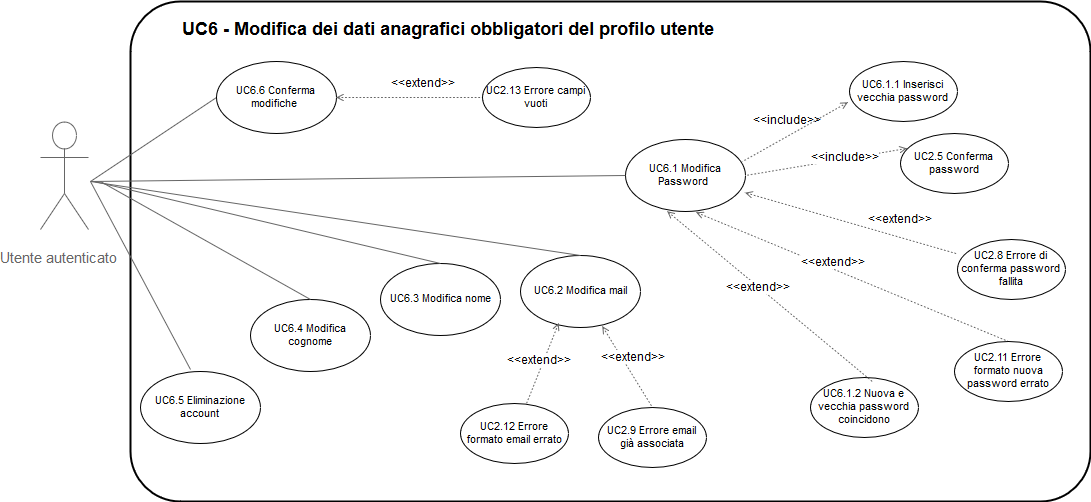
\includegraphics[scale=0.38]{immagini/6.png}
           \caption{Diagramma UC6 - Modifica dei dati anagrafici obbligatori del profilo utente}
           \end{center}
   \end{figure}
     
        
        
    \subsubsection{UC 7-Gestione dati delle macchine utente}
      \begin{itemize}
                \item \textbf{Attori primari}: Utente autenticato;
                \item \textbf{Attori secondari}: Aws;
                 \item \textbf{Scopo e descrizione}: L'utente è in grado di eseguire operazioni di inserimento, modifica e rimozione sulle auto associate al proprio profilo, ovvero le auto che l'utente rende disponibili sulla piattaforma ad altre persone all'interno del sistema per consentire loro di effettuare un viaggio;
                 \item \textbf{Scenario principale}: 
                 \begin{itemize}
                     \item L'utente autenticato accede alla piattaforma;
                     \item L’utente che desidera inserire, rimuovere o modificare auto dal proprio account seleziona la specifica sezione per la gestione delle auto;
                     \item L'utente apporta modifiche secondo le proprie esigenze;
                 \end{itemize}
                 \item \textbf{Scenario secondario} L'utente non desidera continuare l'operazione di inserimento/modifica/eliminazione dell'auto, interrompe il processo e le modifiche non vengono memorizzate dal sistema;
                 \item \textbf{Precondizione}: L'utente autenticato ha scelto di inserire, modificare o rimuovere una vettura all'interno del proprio profilo;
                 \item \textbf{Postcondizione}: Il sistema ha memorizzato le modifiche desiderate e permesse che l'utente ha apportato alla sezione auto.
                 \end{itemize}

       
     \begin{figure}[h!]
           \begin{center}
           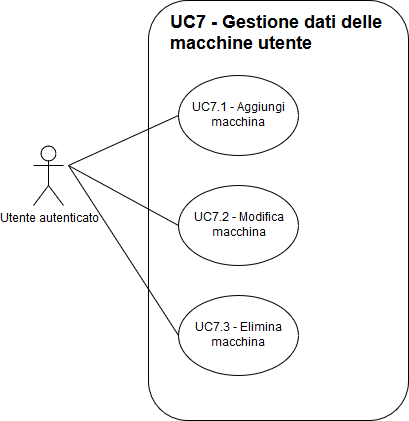
\includegraphics[scale=0.50]{immagini/7.png} 
           \caption{Diagramma UC7 - Gestione dati delle macchine utente}
           \end{center}
        \end{figure}
        
        \newpage
                 
                 \paragraph{UC 7.1-Aggiungi macchina}
                 \begin{itemize}
                \item \textbf{Attori primari}: Utente autenticato;
                
                 \item \textbf{Scopo e descrizione}: L'utente desidera aggiungere un'auto da mettere a disposizione all'interno della piattaforma;
                 \item \textbf{Scenario principale}: L'utente si trova nella sezione di gestione dati della macchina utente e richiede al sistema di inserire un'auto da mettere a disposizione;
                 \item \textbf{Scenario secondario}: L'utente interrompe l'inserimento dei dati e l'aggiunta non viene memorizzata dal sistema.
                
                
                 \item \textbf{Precondizione}: L'utente vuole aggiungere un auto da mettere a disposizione all'interno del sistema;
                 \item \textbf{Postcondizione}: L'utente ha inserito l'auto all'interno del sistema.
                 \end{itemize}
                 
    \subparagraph{UC 7.1.1-Inserimento targa}
    \begin{itemize}
                \item \textbf{Attori primari}: Utente autenticato;
                
                 \item \textbf{Scopo e descrizione}: L'utente compila il campo targa per effettuare la registrazione della propria auto;
                 \item \textbf{Scenario principale}: L'utente si trova nella sezione aggiungi auto e richiede al sistema di inserire la targa della propria macchina;
                 \item \textbf{Estensioni}: 
                 \begin{itemize}
                 \item Il formato della targa inserita non è valido(7.1.12);
                 \item La targa é già associata ad un'altra macchina presente nel sistema(7.1.13).
                 \end{itemize}
                 \item \textbf{Precondizione}: Il sistema fornisce una schermata in cui è possibile inserire la targa della propria auto;
                 \item \textbf{Postcondizione}:L’utente ha compilato il campo "Targa".
                 \end{itemize}
                 
    
                 
    \subparagraph{UC 7.1.2-Inserimento marca}
    \begin{itemize}
                \item \textbf{Attori primari}: Utente autenticato;
                
                 \item \textbf{Scenario principale}: L'utente compila il campo marca per effettuare la registrazione della propria auto;
                 \item \textbf{Scopo e descrizione}: 
                 \begin{itemize}
                     \item L'utente si trova nell'apposita sezione di gestione dati della macchina;
                     \item L'utente compila il campo "Marca".
                 \end{itemize}
                 \item \textbf{Precondizione}: Il sistema fornisce una schermata in cui è possibile inserire la marca dell'auto;
                 \item \textbf{Postcondizione}: L'utente ha compilato il campo "Marca".
                 \end{itemize}
                 
    \subparagraph{UC 7.1.3-Inserimento modello}
    \begin{itemize}
                \item \textbf{Attori primari}: Utente autenticato;
                
                 \item \textbf{Scopo e descrizione}: L'utente compila il campo modello per effettuare la registrazione della propria auto;
                 \item \textbf{Scenario principale}:
                 \begin{itemize}
                     \item L'utente si trova nell'apposita sezione di gestione dati della macchina;
                     \item L'utente compila il campo "Modello".
                 \end{itemize}
                 \item \textbf{Precondizione}: Il sistema fornisce una schermata in cui è possibile inserire il modello dell'auto;
                 \item \textbf{Postcondizione}: L'utente ha compilato il campo "Modello".
                 \end{itemize}
                 
   \subparagraph{UC 7.1.4-Inserimento anno di produzione}
   \begin{itemize}
                \item \textbf{Attori primari}: Utente autenticato;
                
                 \item \textbf{Scopo e descrizione}: L'utente compila il campo anno di produzione per effettuare la registrazione della propria auto;
                 \item \textbf{Scenario principale}: 
                 \begin{itemize}
                     \item L'utente si trova nell'apposita sezione di gestione dati della macchina;
                     \item L'utente compila il campo "Anno di produzione".
                 \end{itemize}
                 \item \textbf{Estensioni}:
                    \begin{itemize}
                        \item L'utente tenta di inserire un formato per l'anno di produzione errato, ovvero minore di zero (UC 7.1.14).
                    \end{itemize}
                 \item \textbf{Precondizione}: Il sistema fornisce una schermata in cui è possibile inserire l'anno di produzione dell'auto;
                 \item \textbf{Postcondizione}: L'utente ha compilato il campo "Anno di produzione".
                 \end{itemize}
                 
    \subparagraph{UC 7.1.5-Inserimento cavalli motore}
    \begin{itemize}
                \item \textbf{Attori primari}: Utente autenticato;
                
                 \item \textbf{Scopo e descrizione}: L'utente compila il campo  cavalli motore per effettuare la registrazione della propria auto;
                 \item \textbf{Scenario principale}: 
                 \begin{itemize}
                     \item L'utente si trova nell'apposita sezione di gestione dati della macchina;
                     \item L'utente compila il campo "Cavalli motore".
                 \end{itemize}
                 \item \textbf{Estensioni}:
                 \begin{itemize} 
                        \item L'utente tenta di inserire un formato per il numero di cavalli motore errato, ovvero minore di zero (UC 7.1.14).
                    \end{itemize}
                 \item \textbf{Precondizione}: Il sistema fornisce una schermata in cui è possibile inserire i cavalli dell'auto;
                 \item \textbf{Postcondizione}: L'utente ha compilato il campo "Cavalli motore".
                 \end{itemize}
                 
                 \subparagraph{UC 7.1.6-Inserimento cilindrata motore}
    \begin{itemize}
                \item \textbf{Attori primari}: Utente autenticato;
               
                 \item \textbf{Scopo e descrizione}: L'utente compila il campo cilindrata motore per effettuare la registrazione della propria auto;
                 \item \textbf{Scenario principale}: 
                 \begin{itemize}
                     \item L'utente si trova nell'apposita sezione di gestione dati della macchina;
                     \item L'utente compila il campo "Cilindrata motore".
                 \end{itemize}
                 \item \textbf{Estensioni}:
                 \begin{itemize}
                        \item L'utente tenta di inserire un formato per la cilindrata del motore errato, ovvero minore di zero (UC 7.1.14).
                    \end{itemize}
                 \item \textbf{Precondizione}: Il sistema fornisce una schermata in cui è possibile inserire la cilindrata dell'auto;
                 \item \textbf{Postcondizione}: L'utente ha compilato il campo "Cilindrata motore".
                 \end{itemize}
                 
                 \subparagraph{UC 7.1.7-Inserimento raggio di percorrenza consentito}
    \begin{itemize}
                \item \textbf{Attori primari}: Utente autenticato;
                
                 \item \textbf{Scopo e descrizione}: L'utente compila il campo raggio motore per effettuare la registrazione della propria auto;
                 \item \textbf{Scenario principale}:
                 \begin{itemize}
                     \item L'utente si trova nell'apposita sezione di gestione dati della macchina;
                     \item L'utente compila il campo "Raggio".
                 \end{itemize}
                 \item \textbf{Estensioni}:
                 \begin{itemize}
                        \item L'utente tenta di inserire un formato per il raggio di produzione consentito errato, ovvero minore di zero (UC 7.1.14).
                    \end{itemize}
                 \item \textbf{Precondizione}: Il sistema fornisce una schermata in cui è possibile inserire il raggio dell'auto;
                 \item \textbf{Postcondizione}: L'utente ha compilato il campo "Raggio".
                 \end{itemize}
                 
        \subparagraph{UC 7.1.8-Inserimento chilometraggio}
    \begin{itemize}
                \item \textbf{Attori primari}: Utente autenticato;
               
                 \item \textbf{Scopo e descrizione}: L'utente compila il campo chilometraggio della macchina per effettuarne la registrazione;
                 \item \textbf{Scenario principale}: L'utente si trova nella sezione aggiungi auto e richiede al sistema di inserire il chilometraggio effettuato dalla propria macchina;
                 \item \textbf{Estensioni}: 
                 \begin{itemize}
                        \item L'utente tenta di inserire un formato per il numero di chilometri effettuati dalla macchina errato, ovvero minore di zero (UC 7.1.14).
                    \end{itemize}
                 \item \textbf{Precondizione}: L'utente desidera inserire il chilometraggio della propria auto;
                 \item \textbf{Postcondizione}:L’utente ha compilato il campo "Chilometri percorsi dall'auto".
                 \end{itemize}
                 
        \subparagraph{UC 7.1.9-Inserimento calendario disponibilità}
    \begin{itemize}
                \item \textbf{Attori primari}: Utente autenticato;
              
                 \item \textbf{Scopo e descrizione}: L'utente compila il campo calendario disponibilità per effettuare la registrazione della propria auto;
                 \item \textbf{Scenario principale}: L'utente si trova nella sezione aggiungi auto e richiede al sistema di inserire il calendario relativo alla propria macchina;
                 
                 \item \textbf{Precondizione}: L'utente desidera inserire il calendario di disponibilità della propria auto;
                 \item \textbf{Postcondizione}:L’utente ha compilato il campo "Calendario disponibilità".
                 \end{itemize}
                 
                 
            \subparagraph{UC 7.1.10-Inserimento tariffa oraria}
    \begin{itemize}
                \item \textbf{Attori primari}: Utente autenticato;
               
                 \item \textbf{Scopo e descrizione}: L'utente compila il campo tariffa oraria per effettuare la registrazione della propria auto;
                 \item \textbf{Scenario principale}: L'utente si trova nella sezione aggiungi auto e richiede al sistema di inserire la tariffa oraria relativa alla propria macchina;
                 \item \textbf{Estensioni}:
                    \begin{itemize}
                        \item L'utente tenta di inserire un formato per la tariffa oraria errato, ovvero minore di zero (UC 7.1.14).
                    \end{itemize}
                 \item \textbf{Precondizione}: L'utente desidera inserire la tariffa oraria della propria auto;
                 \item \textbf{Postcondizione}:L’utente compila il campo "Tariffa oraria".
                 \end{itemize}
                 
                 
                 
            \subparagraph{UC 7.1.11-Visualizzazione messaggio errore campi di compilazione vuoti}
    \begin{itemize}
                \item \textbf{Attori primari}: Utente autenticato;
               
                 \item \textbf{Scopo e descrizione}: La procedura di registrazione ha riscontrato un errore in merito ai
                dati inseriti. Nello specifico l'errore è dovuto al fatto che esiste almeno un campo di compilazione lasciato vuoto.
                 \item \textbf{Scenario principale}: 
                 \begin{itemize}
                     \item L'utente ha inserito i dati per la registrazione della macchina;
                     \item L'utente non ha compilato uno o più campi.
                 \end{itemize}
                 \item \textbf{Precondizione}: L'utente ha inserito i dati della sua auto e ha confermato la registrazione. L'utente tenta di aggiungere la propria auto non compilando tutti i campi.
                 \item \textbf{Postcondizione}: Viene notificato all'utente che si è verificato un errore in merito alla procedura di aggiungere un auto. L'utente ora è consapevole del fatto che deve compilare tutti i campi per aggiungere un auto.
                 \end{itemize}
                 
                 
                \subparagraph{UC 7.1.12-Visualizzazione messaggio errore formato targa non valido} 
    \begin{itemize}
                \item \textbf{Attori primari}: Utente autenticato;
               
                 \item \textbf{Scopo e descrizione}: La procedura di inserimento della targa ha riscontrato un errore perché il formato non è valido, quindi:
                
              
                 \item \textbf{Scenario principale}: 
                 \begin{itemize}
                     \item L'utente ha inserito la targa;
                     \item Il formato della targa inserita nel campo "Targa" non è corretto, pertanto viene scatenato un errore.
                 \end{itemize}
                 \item \textbf{Precondizione}:  L'utente tenta di aggiungere un auto avente il formato della targa errato.
                 \item \textbf{Postcondizione}: Viene notificato all'utente che si è verificato un errore in merito alla registrazione dell'auto. L'utente ora è consapevole del fatto che il formato della targa inserita non è consentito.
                 \end{itemize}
                 
                 \subparagraph{UC 7.1.13-Visualizzazione messaggio errore targa già esistente}
    \begin{itemize}
                \item \textbf{Attori primari}: Utente autenticato;
               
                 \item \textbf{Scopo e descrizione}: La procedura di registrazione dell'auto ha riscontrato un errore in merito ai dati inseriti. Nello specifico l'errore è dovuto al fatto che la targa inserita nel campo "Targa" è già associata a un'altra macchina presente nella piattaforma.
                 \item \textbf{Scenario principale}:
                 \begin{itemize}
                     \item L'utente ha inserito i dati della propria macchina per metterla a disposizione;
                     \item La targa inserita nel campo "Targa" è associata a un'altra macchina,pertanto viene scatenato un errore.
                 \end{itemize}
                 \item \textbf{Precondizione}: L'utente ha inserito tutti i dati per la registrazione dell'auto. L'utente tenta di registrare la macchina usando una targa già esistente.
                 \item \textbf{Postcondizione}: Viene notificato all'utente che si è verificato un errore in merito alla procedura di registrazione. L’utente ora è consapevole del fatto che la targa inserita è già associata ad un'altra macchina.
                 \end{itemize}
                 
                 
                 \subparagraph{UC 7.1.14-Visualizzazione messaggio errore campo minore di zero} 
    \begin{itemize}
                \item \textbf{Attori primari}: Utente autenticato;
               
                 \item \textbf{Scopo e descrizione}: Durante la procedura di inserimento dei dati si è sollevata una condizione di errore. Nel particolare l'errore si può riscontrare in uno dei seguenti campi: anno di produzione, cavalli motore, cilindrata del motore, raggio di percorrenza consentito o chilometri effettuati dall'auto. La procedura di inserimento ha riscontrato un errore perché il formato inserito in almeno uno dei campi non è valido, ovvero si inserisce un numero minore di zero.
                 \item \textbf{Scenario principale}: 
                 \begin{itemize}
                     \item L'utente ha inserito i dati di anno di produzione, cavalli motore, cilindrata del motore, raggio di percorrenza consentito e chilometri fatti;
                     \item Il formato di almeno uno di questi campi è minore di zero, quindi non corretto. Viene scatenato un errore.
                 \end{itemize}
                 \item \textbf{Precondizione}: L'utente ha inserito i dati della macchina per poterla mettere a disposizione. L'utente tenta di aggiungere un auto avente il formato di almeno uno dei campi sopracitati errato.
                 \item \textbf{Postcondizione}: Viene notificato all'utente che si è verificato un errore in merito all'aggiunta dell'auto. L'utente ora è consapevole del fatto che il formato di almeno uno dei campi sopracitati non è consentito.
                 \end{itemize}
         
         \subparagraph{UC 7.1.15-Conferma aggiunta dell'auto}
            \begin{itemize}
                \item \textbf{Attori primari}: Utente autenticato;
                
                \item \textbf{Scopo e descrizione}: L'utente conferma l' operazione di aggiunta dell'auto al proprio profilo; 
                \item \textbf{Scenario principale}:
                    \begin{itemize}
                        \item L'utente si trova nella sezione dedicata all'aggiunta di un'auto all'interno del proprio profilo;
                        \item L'utente conferma l'operazione di aggiunta cliccando il pulsante apposito.
                    \end{itemize}
                \item \textbf{Estensioni}: La registrazione può fallire a causa del seguente errore di compilazione da parte dell'utente:
                \begin{itemize}
                \item Esistono dei campi vuoti (UC 7.1.11).
                \end{itemize}
                \item \textbf{Precondizione}: L'utente si trova in una schermata in cui è possibile dare la conferma
                dei dati inseriti per l'aggiunta dell'auto all'interno del proprio profilo;
                \item \textbf{Postcondizione}:L’utente ha espresso di voler procedere con la conferma dell'operazione e quindi il sistema memorizza la decisione.
            \end{itemize}
                        
                 
                 
           \begin{figure}[h!]
           \begin{center}
           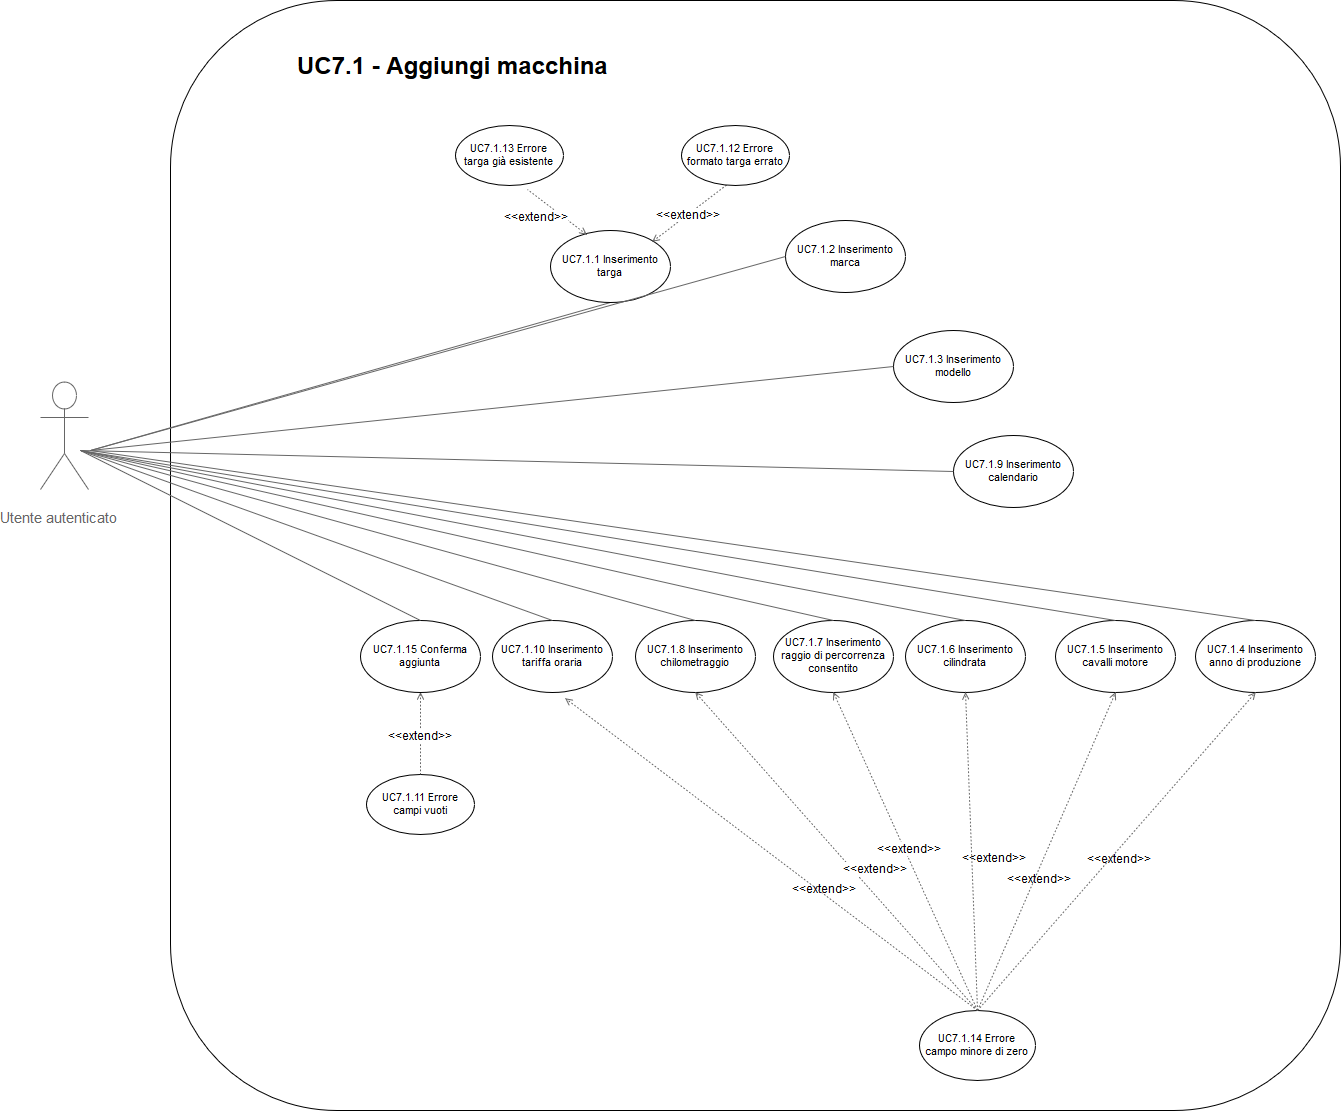
\includegraphics[scale=0.3]{immagini/71.png}   
           \caption{Diagramma UC7.1 - Aggiungi macchina}
           \end{center}
           \end{figure}      
           
           \newpage      
                       
                     
    \paragraph{UC 7.2-Modifica macchina}
    \begin{itemize}
                \item \textbf{Attori primari}: Utente autenticato;
                
                 \item \textbf{Scopo e descrizione}: L'utente desidera modificare un'auto all'interno del proprio profilo da mettere a disposizione;
                 \item \textbf{Scenario principale}:
                 \begin{itemize}
                    \item L'utente autenticato accede alla piattaforma;
                    \item L'utente che desidera apportare modifiche al proprio veicolo seleziona la specifica sezione indicante il proprio parco macchine;
                    \item L'utente seleziona l'auto da modificare;
                    \item L'utente modifica i propri dati secondo esigenze;
                    \item L'utente conferma le modifiche apportate.
                \end{itemize}
                \item \textbf{Scenario secondario}: L'utente interrompe l'inserimento delle modifiche sui dati e le modifiche non vengono memorizzate dal sistema.
                
                 \item \textbf{Precondizione}: L'utente ha già inserito almeno un auto all'interno del proprio profilo e vuole modificare una delle macchine da mettere a disposizione all'interno del sistema;
                 \item \textbf{Postcondizione}: L'utente ha modificato l'auto all'interno del sistema.
                 \end{itemize}
    
    \subparagraph{UC 7.2.1-Selezione macchina da modificare}
    \begin{itemize}
                \item \textbf{Attori primari}: Utente autenticato;
               
                 \item \textbf{Scopo e descrizione}: L’utente seleziona l'auto (tra quelle da lui precedentemente inserite all'interno del proprio account) sulla quale vuole effettuare l'operazione di modifica dei dati;
                 \item \textbf{Scenario principale}: 
                 \begin{itemize}
                     \item L’utente si trova nella sezione dedicata alla modifica dei dati relativi alle macchine dell'utente;
                     \item L'utente seleziona una delle macchine associate al suo account sulla quale vuole eseguire l'operazione di modifica.          \end{itemize}
                 \item \textbf{Precondizione}: L’utente si trova in una schermata in cui selezionare su quale macchina è possibile effettuare l'operazione di modifica;
                 \item \textbf{Postcondizione}: L’utente seleziona l'auto sulla quale vuole effettuare la modifica dei relativi dati (targa, marca, modello, anno di produzione, cavalli motore, cilindrata, raggio consentito, kilometraggio, calendario disponibilità o tariffa oraria).
                 \end{itemize}
    
    \subparagraph{UC 7.2.2-Conferma modifica}
    \begin{itemize}
                \item \textbf{Attori primari}: Utente autenticato;;
                
                 \item \textbf{Scopo e descrizione}: L’utente conferma le modifiche inserite precedentemente per permettere al sistema di memorizzarle;
                 \item \textbf{Scenario principale}: 
                 \begin{itemize}
                     \item L’utente si trova nella sezione dedicata alla modifica dei dati relativi alle macchine dell'utente;
                     \item L'utente conferma l'operazione di modifica cliccando il pulsante apposito. 
                 \end{itemize}
                 \item \textbf{Estensioni}:
            \begin{itemize}
                \item Le modifiche non vengono salvate nel caso l'utente lasci dei campi di compilazione vuoti (UC 7.1.11).
            \end{itemize}
                 \item \textbf{Precondizione}: L’utente si trova in una schermata in cui è possibile dare la conferma dell'operazione di modifica;
                 \item \textbf{Postcondizione}: L’utente ha espresso di voler procedere con la conferma e quindi con la modifica ai propri dati.
                 \end{itemize}
                 
    \subparagraph{UC 7.2.3-Modifica targa}
            \begin{itemize}
                \item \textbf{Attori primari}: Utente autenticato;
                
                \item \textbf{Scopo e descrizione}: L'utente seleziona una delle auto associate al proprio account e ne modifica il numero di targa; 
                \item \textbf{Scenario principale}:
                    \begin{itemize}
                        \item L'utente si trova nella sezione dedicata alla modifica dei dati relativi alle macchine precedentemente inserite dall'utente nel suo account personale;
                        \item L'utente autenticato ha selezionato una delle auto da lui messe a disposizione sulla quale desidera effettuare l'operazione di modifica;
                        \item L'utente modifica la targa relativa a una determinata macchina dell'account.
                    \end{itemize}
                \item \textbf{Scenario secondario}: L'utente non desidera continuare con l'operazione di modifica. Le modifiche pertanto non vengono salvate;
                \item \textbf{Estensioni}:
                    \begin{itemize}
                        \item La nuova targa inserita non è nel formato corretto (UC 7.1.12);
                        \item La nuova targa inserita è già associata ad un'altra macchina presente nel sistema (UC 7.1.13).
                    \end{itemize}
                \item \textbf{Precondizione}: L'utente si trova in una schermata in cui è possibile modificare i dati relativi alla targa di una delle auto associate all'account, precedentemente selezionata;
                \item \textbf{Postcondizione}:L'utente modifica il numero di targa associato a una delle macchine del suo account.
            \end{itemize}
    
    
    \subparagraph{UC 7.2.4-Modifica marca}
            \begin{itemize}
                \item \textbf{Attori primari}: Utente autenticato;
               
                \item \textbf{Scopo e descrizione}: L'utente seleziona una delle auto associate al proprio account e ne modifica la marca; 
                \item \textbf{Scenario principale}:
                    \begin{itemize}
                        \item L'utente si trova nella sezione dedicata alla modifica dei dati relativi alle macchine precedentemente inserite dall'utente nel suo account personale;
                        \item L'utente autenticato ha selezionato una delle auto da lui messe a disposizione sulla quale desidera effettuare l'operazione di modifica;
                        \item L'utente modifica la marca relativa a una determinata macchina dell'account.
                    \end{itemize}
                \item \textbf{Scenario secondario}: L'utente non desidera continuare con l'operazione di modifica. Le modifiche pertanto non vengono salvate;
        
                \item \textbf{Precondizione}: L'utente si trova in una schermata in cui è possibile modificare i dati relativi alla marca di una delle auto associate all'account, precedentemente selezionata;
                \item \textbf{Postcondizione}:L'utente modifica la marca associata a una delle macchine del suo account.
            \end{itemize}
    
    \subparagraph{UC 7.2.5-Modifica modello}
            \begin{itemize}
                \item \textbf{Attori primari}: Utente autenticato;
               
                \item \textbf{Scopo e descrizione}: L'utente seleziona una delle auto associate al proprio account e ne modifica il modello; 
                \item \textbf{Scenario principale}:
                    \begin{itemize}
                        \item L'utente si trova nella sezione dedicata alla modifica dei dati relativi alle macchine precedentemente inserite dall'utente nel suo account personale;
                        \item L'utente autenticato ha selezionato una delle auto da lui messe a disposizione sulla quale desidera effettuare l'operazione di modifica;
                        \item L'utente modifica il modello relativo a una determinata macchina dell'account.
                    \end{itemize}
                \item \textbf{Scenario secondario}: L'utente non desidera continuare con l'operazione di modifica. Le modifiche pertanto non vengono salvate;
        
                \item \textbf{Precondizione}: L'utente si trova in una schermata in cui è possibile modificare i dati relativi al modello di una delle auto associate all'account, precedentemente selezionata;
                \item \textbf{Postcondizione}:L'utente modifica il modello associata a una delle macchine del suo account.
            \end{itemize}
            
            
            \subparagraph{UC 7.2.6-Modifica anno di produzione}
            \begin{itemize}
                \item \textbf{Attori primari}: Utente autenticato;
                
                \item \textbf{Scopo e descrizione}: L'utente seleziona una delle auto associate al proprio account e ne modifica l'anno di produzione; 
                \item \textbf{Scenario principale}:
                    \begin{itemize}
                        \item L'utente si trova nella sezione dedicata alla modifica dei dati relativi alle macchine precedentemente inserite dall'utente nel suo account personale;
                        \item L'utente autenticato ha selezionato una delle auto da lui messe a disposizione sulla quale desidera effettuare l'operazione di modifica;
                        \item L'utente modifica l'anno di produzione relativo a una determinata macchina dell'account.
                    \end{itemize}
                \item \textbf{Scenario secondario}: L'utente non desidera continuare con l'operazione di modifica. Le modifiche pertanto non vengono salvate;
                \item \textbf{Estensioni}:
                    \begin{itemize}
                        \item Viene sollevato un errore nel caso l'utente tenti di aggiornare l'anno di produzione dell'auto in un formato non corretto, ovvero minore di zero (UC 7.1.14); 
                    \end{itemize}
                \item \textbf{Precondizione}: L'utente si trova in una schermata in cui è possibile modificare i dati relativi all'anno di produzione di una delle auto associate all'account, precedentemente selezionata;
                \item \textbf{Postcondizione}:L'utente modifica l'anno di produzione associato a una delle macchine del suo account.
            \end{itemize}
            
            
            \subparagraph{UC 7.2.7-Modifica cavalli motore}
            \begin{itemize}
                \item \textbf{Attori primari}: Utente autenticato;
              
                \item \textbf{Scopo e descrizione}: L'utente seleziona una delle auto associate al proprio account e ne modifica i cavalli motore; 
                \item \textbf{Scenario principale}:
                    \begin{itemize}
                        \item L'utente si trova nella sezione dedicata alla modifica dei dati relativi alle macchine precedentemente inserite dall'utente nel suo account personale;
                        \item L'utente autenticato ha selezionato una delle auto da lui messe a disposizione sulla quale desidera effettuare l'operazione di modifica;
                        \item L'utente modifica i cavalli motore relativi a una determinata macchina dell'account.
                    \end{itemize}
                \item \textbf{Scenario secondario}: L'utente non desidera continuare con l'operazione di modifica. Le modifiche pertanto non vengono salvate;
                \item \textbf{Estensioni}:
                    \begin{itemize}
                        \item Viene sollevato un errore nel caso l'utente tenti di aggiornare il numero di cavalli motore dell'auto in un formato non corretto, ovvero minore di zero (UC 7.1.14); 
                    \end{itemize}
                \item \textbf{Precondizione}: L'utente si trova in una schermata in cui è possibile modificare i dati relativi ai cavalli motore di una delle auto associate all'account, precedentemente selezionata;
                \item \textbf{Postcondizione}:L'utente modifica i cavalli motore associati a una delle macchine del suo account.
            \end{itemize}
            
            
            
            \subparagraph{UC 7.2.8-Modifica cilindrata motore}
            \begin{itemize}
                \item \textbf{Attori primari}: Utente autenticato;
                
                \item \textbf{Scopo e descrizione}: L'utente seleziona una delle auto associate al proprio account e ne modifica la cilindrata del motore; 
                \item \textbf{Scenario principale}:
                    \begin{itemize}
                        \item L'utente si trova nella sezione dedicata alla modifica dei dati relativi alle macchine precedentemente inserite dall'utente nel suo account personale;
                        \item L'utente autenticato ha selezionato una delle auto da lui messe a disposizione sulla quale desidera effettuare l'operazione di modifica;
                        \item L'utente modifica la cilindrata del motore relativa a una determinata macchina dell'account.
                    \end{itemize}
                \item \textbf{Scenario secondario}: L'utente non desidera continuare con l'operazione di modifica. Le modifiche pertanto non vengono salvate;
                \item \textbf{Estensioni}:
                    \begin{itemize}
                        \item Viene sollevato un errore nel caso l'utente tenti di aggiornare la cilindrata del motore dell'auto in un formato non corretto, ovvero minore di zero (UC 7.1.14); 
                    \end{itemize}
                \item \textbf{Precondizione}: L'utente si trova in una schermata in cui è possibile modificare i dati relativi alla cilindrata del motore di una delle auto associate all'account, precedentemente selezionata;
                \item \textbf{Postcondizione}:L'utente modifica la cilindrata del motore associata ad una delle macchine del suo account.
            \end{itemize}
                 
                 
                 
            \subparagraph{UC 7.2.9-Modifica raggio di percorrenza}
            \begin{itemize}
                \item \textbf{Attori primari}: Utente autenticato;
                
                \item \textbf{Scopo e descrizione}: L'utente seleziona una delle auto associate al proprio account e ne modifica il raggio di percorrenza consentito; 
                \item \textbf{Scenario principale}:
                    \begin{itemize}
                        \item L'utente si trova nella sezione dedicata alla modifica dei dati relativi alle macchine precedentemente inserite dall'utente nel suo account personale;
                        \item L'utente autenticato ha selezionato una delle auto da lui messe a disposizione sulla quale desidera effettuare l'operazione di modifica;
                        \item L'utente modifica il raggio di percorrenza consentito relativo a una determinata macchina dell'account.
                    \end{itemize}
                \item \textbf{Scenario secondario}: L'utente non desidera continuare con l'operazione di modifica. Le modifiche pertanto non vengono salvate;
                \item \textbf{Estensioni}:
                    \begin{itemize}
                        \item Viene sollevato un errore nel caso l'utente tenti di aggiornare il raggio di percorrenza consentito in un formato non corretto, ovvero minore di zero (UC 7.1.14); 
                    \end{itemize}
                \item \textbf{Precondizione}: L'utente si trova in una schermata in cui è possibile modificare i dati relativi al raggio di percorrenza consentito a una delle auto associate all'account, precedentemente selezionata;
                \item \textbf{Postcondizione}:L'utente modifica il raggio di percorrenza consentito associato a una delle macchine del suo account.
            \end{itemize}
            
            \subparagraph{UC 7.2.10-Modifica chilometri percorsi dall'auto}
            \begin{itemize}
                \item \textbf{Attori primari}: Utente autenticato;
              
                \item \textbf{Scopo e descrizione}: L'utente seleziona una delle auto associate al proprio account e ne modifica i chilometri percorsi; 
                \item \textbf{Scenario principale}:
                    \begin{itemize}
                        \item L'utente si trova nella sezione dedicata alla modifica dei dati relativi alle macchine precedentemente inserite dall'utente nel suo account personale;
                        \item L'utente autenticato ha selezionato una delle auto da lui messe a disposizione sulla quale desidera effettuare l'operazione di modifica;
                        \item L'utente modifica i chilometri percorsi relativi a una determinata macchina dell'account.
                    \end{itemize}
                \item \textbf{Scenario secondario}: L'utente non desidera continuare con l'operazione di modifica. Le modifiche pertanto non vengono salvate;
                \item \textbf{Estensioni}:
                    \begin{itemize}
                        \item Viene sollevato un errore nel caso l'utente tenti di aggiornare i chilometri effettuati dell'auto in un formato non corretto, ovvero minore di zero (UC 7.1.14); 
                    \end{itemize}
                \item \textbf{Precondizione}: L'utente si trova in una schermata in cui è possibile modificare i dati relativi ai chilometri percorsi di una delle auto associate all'account, precedentemente selezionata;
                \item \textbf{Postcondizione}:L'utente modifica i chilometri percorsi da una delle macchine del suo account.
            \end{itemize}
            
        \subparagraph{UC 7.2.11-Modifica calendario disponibilità dell'auto}
            \begin{itemize}
                \item \textbf{Attori primari}: Utente autenticato;
               
                \item \textbf{Scopo e descrizione}: L'utente seleziona una delle auto associate al proprio account e ne modifica il calendario di disponibilità; 
                \item \textbf{Scenario principale}:
                    \begin{itemize}
                        \item L'utente si trova nella sezione dedicata alla modifica dei dati relativi alle macchine precedentemente inserite dall'utente nel suo account personale;
                        \item L'utente autenticato ha selezionato una delle auto da lui messe a disposizione sulla quale desidera effettuare l'operazione di modifica;
                        \item L'utente modifica il calendario di disponibilità relativo a una determinata macchina dell'account.
                    \end{itemize}
                \item \textbf{Scenario secondario}: L'utente non desidera continuare con l'operazione di modifica. Le modifiche pertanto non vengono salvate;

                \item \textbf{Precondizione}: L'utente si trova in una schermata in cui è possibile modificare i dati relativi al calendario di disponibilità  di una delle auto associate all'account, precedentemente selezionata;
                \item \textbf{Postcondizione}:L'utente modifica il calendario di disponibilità percorsi da una delle macchine del suo account.
            \end{itemize}
            
        \subparagraph{UC 7.2.12-Modifica tariffa oraria dell'auto}
            \begin{itemize}
                \item \textbf{Attori primari}: Utente autenticato;
               
                \item \textbf{Scopo e descrizione}: L'utente seleziona una delle auto associate al proprio account e ne modifica la tariffa oraria; 
                \item \textbf{Scenario principale}:
                    \begin{itemize}
                        \item L'utente si trova nella sezione dedicata alla modifica dei dati relativi alle macchine precedentemente inserite dall'utente nel suo account personale;
                        \item L'utente autenticato ha selezionato una delle auto da lui messe a disposizione sulla quale desidera effettuare l'operazione di modifica;
                        \item L'utente modifica il la tariffa oraria relativa a una determinata macchina dell'account.
                    \end{itemize}
                \item \textbf{Scenario secondario}: L'utente non desidera continuare con l'operazione di modifica. Le modifiche pertanto non vengono salvate;
                \item \textbf{Estensioni}:
                    \begin{itemize}
                        \item Viene sollevato un errore nel caso l'utente tenti di aggiornare la cilindrata del motore dell'auto in un formato non corretto, ovvero minore di zero (UC 7.1.14); 
                    \end{itemize}
                \item \textbf{Precondizione}: L'utente si trova in una schermata in cui è possibile modificare i dati relativi alla tariffa oraria di una delle auto associate all'account, precedentemente selezionata;
                \item \textbf{Postcondizione}:L'utente modifica la tariffa oraria di una delle macchine del suo account.
            \end{itemize}
    
    
    \begin{figure}[h!]
           \begin{center}
           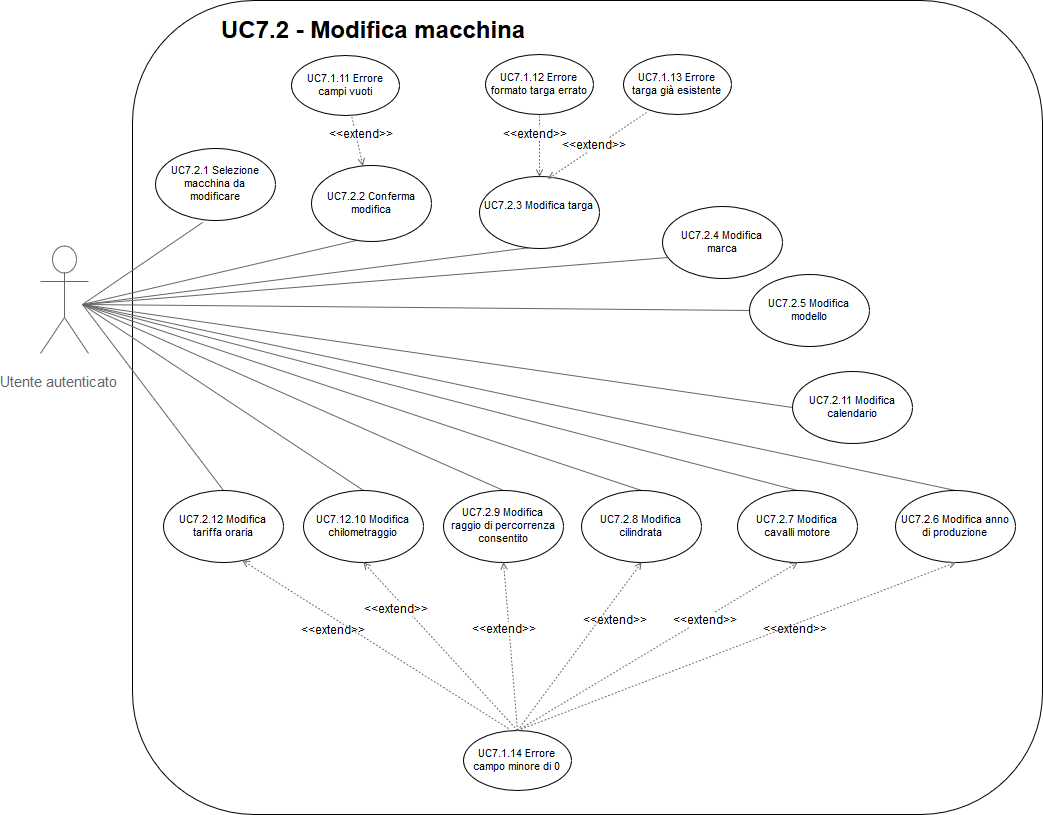
\includegraphics[scale=0.35]{immagini/72.png}    
           \caption{Diagramma UC7.2 - Modifica macchina}
           \end{center}
           \end{figure}  
            
    \newpage
    
    \paragraph{UC 7.3-Eliminazione macchina}
    \begin{itemize}
                \item \textbf{Attori primari}: Utente autenticato;
               
                 \item \textbf{Scopo e descrizione}: L'utente desidera cancellare una o più auto associate al proprio profilo sulla piattaforma;
                 \item \textbf{Scenario principale}: 
                 \begin{itemize}
                     \item L'utente si trova nella sezione dedicata alla cancellazione dell'auto;
                     \item L'utente conferma la cancellazione dell'auto.
                 \end{itemize}
                 \item \textbf{Scenario secondario}: L'utente interrompe il processo e l'eliminazione non viene memorizzata dal sistema.
                 \item \textbf{Precondizione}: L'utente si trova in una schermata in cui è possibile cancellare un auto precedentemente aggiunta;
                 \item \textbf{Postcondizione}: L'utente ha espresso di voler procedere con la cancellazione e quindi il sistema cancella la macchina selezionata.
                 \end{itemize}
                 
          
        
        
    \subsubsection{UC 8-Ricerca macchina}
       \begin{itemize}
        \item \textbf{Attori primari}: Utente autenticato;
        \item \textbf{Attori secondari}: Aws;
        \item \textbf{Scopo e descrizione}: L'utente desidera effettuare un viaggio, pertanto ricerca le auto disponibili sulla piattaforma per percorrere il proprio itinerario.
        \item \textbf{Scenario principale}:
            \begin{itemize}
                \item L'utente ha effettuato l'accesso all'interno del sistema;
                \item L'utente che desidera effettuare la ricerca si posiziona nell'apposita sezione "Cerca".
            \end{itemize}
        
        \item \textbf{Scenario secondario}: L'utente non desidera procedere con la ricerca: smette di compilare i campi richiesti e la ricerca viene interrotta.
       
        
       
        \item \textbf{Precondizione}: L'utente è autenticato all'interno del sistema e si posiziona nella sezione di ricerca.
        \item \textbf{Postcondizione}: L'utente effettua una ricerca e visualizza le offerte di macchine disponibili.
        \end{itemize}
            
      \paragraph{UC 8.1-Inserimento delle zone coperte dal viaggio }
       \begin{itemize}
        \item \textbf{Attori primari}: Utente autenticato;
        
        \item \textbf{Scopo e descrizione}: L'utente autenticato desidera ricercare le auto disponibili per effettuare un viaggio. Per farlo seleziona le aree del viaggio che deve percorrere.
        \item \textbf{Scenario principale}:
            \begin{itemize}
                \item L'utente ha effettuato l'accesso all'interno del sistema;
                \item L'utente che desidera effettuare la ricerca si posiziona nell'apposita sezione "Cerca";
                \item L'utente seleziona le aree che deve percorrere con il suo viaggio.
            \end{itemize}
        
        \item \textbf{Precondizione}: L'utente è autenticato all'interno del sistema e si posiziona nella sezione di ricerca.
        \item \textbf{Postcondizione}: L'utente posizionato nella sezione di ricerca inserisce i dati relativi alle zone del viaggio e il sistema memorizza le scelte.
        \end{itemize}
        
        
        
        
         \paragraph{UC 8.2-Inserimento dei giorni nei quali effettuare il viaggio}
       \begin{itemize}
        \item \textbf{Attori primari}: Utente autenticato;
       
        \item \textbf{Scopo e descrizione}: L'utente autenticato desidera ricercare le auto disponibili per effettuare un viaggio; per farlo seleziona i giorni in cui deve eseguire il viaggio.
        \item \textbf{Scenario principale}:
            \begin{itemize}
                \item L'utente ha effettuato l'accesso all'interno del sistema;
                \item L'utente che desidera effettuare la ricerca si posiziona nell'apposita sezione "Cerca";
                \item L'utente seleziona i giorni in cui deve percorrere con il suo viaggio.
            \end{itemize}
        
        \item \textbf{Precondizione}: L'utente è autenticato all'interno del sistema e si posiziona nella sezione di ricerca.
        \item \textbf{Postcondizione}: L'utente posizionato nella sezione di ricerca inserisce i dati relativi ai giorni in cui vuole svolgere il viaggio e il sistema memorizza le scelte.
        \end{itemize}
        
        
        \paragraph{UC 8.3-Inserimento prezzo massimo desiderato per il viaggio}
       \begin{itemize}
        \item \textbf{Attori primari}: Utente autenticato;
       
        \item \textbf{Scopo e descrizione}: L'utente autenticato desidera ricercare le auto disponibili per effettuare un viaggio; per farlo seleziona il prezzo massimo che vuole pagare per il viaggio.
        \item \textbf{Scenario principale}:
            \begin{itemize}
                \item L'utente ha effettuato l'accesso all'interno del sistema;
                \item L'utente che desidera effettuare la ricerca si posiziona nell'apposita sezione "Cerca";
                \item L'utente seleziona il prezzo che desidera pagare per il viaggio.
            \end{itemize}
        
        \item \textbf{Precondizione}: L'utente è autenticato all'interno del sistema e si posiziona nella sezione di ricerca.
        \item \textbf{Postcondizione}: L'utente posizionato nella sezione di ricerca inserisce i dati relativi al prezzo massimo che desidera pagare per il viaggio e il sistema memorizza le scelte.
        \end{itemize}
        
        
        \paragraph{UC 8.4-Inserimento delle caratteristiche dell'auto con la quale effettuare il viaggio}
       \begin{itemize}
        \item \textbf{Attori primari}: Utente autenticato;
      
        \item \textbf{Scopo e descrizione}: L'utente autenticato desidera ricercare le auto disponibili per effettuare un viaggio; per farlo seleziona le caratteristiche che desidera per l'auto.
        \item \textbf{Scenario principale}:
            \begin{itemize}
                \item L'utente ha effettuato l'accesso all'interno del sistema;
                \item L'utente che desidera effettuare la ricerca si posiziona nell'apposita sezione "Cerca";
                \item L'utente seleziona le caratteristiche volute per l'auto utilizzata per il viaggio.
            \end{itemize}
        
        \item \textbf{Precondizione}: L'utente è autenticato all'interno del sistema e si posiziona nella sezione di ricerca.
        \item \textbf{Postcondizione}: L'utente posizionato nella sezione di ricerca inserisce i dati della macchina da utilizzare per il viaggio e il sistema memorizza le scelte.
        \end{itemize}
        
        
        \paragraph{UC 8.5-Conferma ricerca}
            \begin{itemize}
                \item \textbf{Attori primari}: : Utente autenticato;
                
                \item \textbf{Scopo e descrizione}: L'utente conferma di voler effettuare la ricerca con i dati inseriti precedentemente. 
                \item \textbf{Scenario principale}:
                    \begin{itemize}
                        \item L'utente si trova nella sezione dedicata alla ricerca;
                        \item L'utente conferma l'operazione di ricerca cliccando il pulsante apposito.
                    \end{itemize}
                    \item \textbf{Estensioni}: 
            \begin{itemize}
                \item Nel caso il formato dei campi compilati non sia conforme al formato richiesto viene visualizzato un messaggio di errore (UC 8.6).
            \end{itemize}
                \item \textbf{Precondizione}:L'utente si trova in una schermata in cui è possibile dare la conferma dei dati inseriti su cui eseguire la ricerca;
                \item \textbf{Postcondizione}:L’utente ha espresso di voler procedere con la conferma e quindi con la ricerca all'interno del sistema.
            \end{itemize}
        
        
        
        \paragraph{UC 8.6-Errore formato compilazione campi}
       \begin{itemize}
        \item \textbf{Attori primari}: Utente autenticato;
        \item \textbf{Scopo e descrizione}:  La procedura di ricerca ha riscontrato un errore in merito ai dati inseriti durante la procedura. Nello specifico l'errore è dovuto al fatto che esiste almeno un campo di compilazione con formato non congruo.
        \item \textbf{Scenario principale}:
            \begin{itemize}
                \item L'utente ha effettuato l'accesso all'interno del sistema;
                \item L'utente ha compilato tutti i campi per la ricerca. Almeno uno di questi non è nel formato richiesto, quindi viene scatenato un errore.
            \end{itemize}
        \item \textbf{Precondizione}: L'utente ha compilato i campi di interesse e ha confermato l'operazione. L'utente tenta di effettuare la ricerca inserendo almeno un formato per i campi non consentito.
        \item \textbf{Postcondizione}: L'utente non è in grado di effettuare la ricerca a causa dell'errore scatenato.
        \end{itemize}
  
  \begin{figure}[h!]
           \begin{center}
           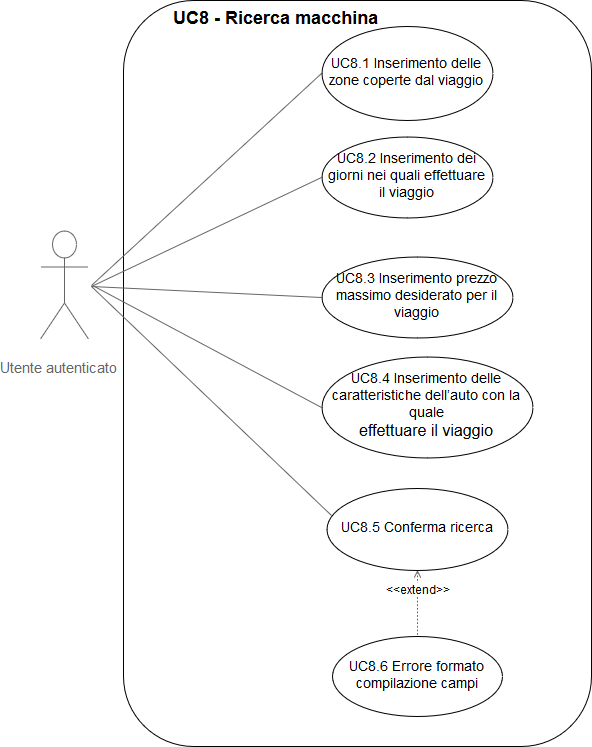
\includegraphics[scale=0.60]{immagini/8.png}    
           \caption{Diagramma UC8 - Ricerca macchina}
           \end{center}
    \end{figure}  
  
  
        
        \subsubsection{UC 9-Prenotazione viaggio}
       \begin{itemize}
        \item \textbf{Attori primari}: Utente autenticato;
        \item \textbf{Attori secondari}: Aws;
        \item \textbf{Scopo e descrizione}: L'utente autenticato desidera prenotare un viaggio utilizzando una delle macchine disponibile per compiere il suo itinerario.
        \item \textbf{Scenario principale}:
            \begin{itemize}
                \item L'utente ha effettuato l'accesso all'interno del sistema;
                \item L'utente ha effettuato una ricerca all'interno del sistema secondo alcuni parametri per ricercare un'auto con cui effettuare un viaggio;
                \item L'utente visualizza i risultati delle macchine che rispondono alle richieste espresse in fase di ricerca da parte dell'utente;
                \item L'utente che desidera effettuare la prenotazione del viaggio seleziona la macchina disponibile che gli interessa;
                \item Una volta selezionata l'utente è in grado di confermare la prenotazione.
            \end{itemize}
        
        \item \textbf{Scenario secondario}: L'utente non desidera procedere con la prenotazione: non seleziona nessuna auto e la prenotazione viene interrotta.
        
        \item \textbf{Precondizione}: L'utente è autenticato all'interno del sistema ed ha effettuato una ricerca. Visualizza i risultati relativi alla ricerca e da qui sceglie una macchina che si adegua alle sue esigenze di viaggio.
        \item \textbf{Postcondizione}: L'utente ha prenotato l'auto per svolgere un determinato viaggio.
        \end{itemize}  
        
        \paragraph{UC 9.1-Selezione macchina}
    \begin{itemize}
                \item \textbf{Attori primari}: Utente autenticato;
                
                 \item \textbf{Scopo e descrizione}: L’utente seleziona una tra le auto che rispondono alla ricerca effettuata;
                 \item \textbf{Scenario principale}: 
                 \begin{itemize}
                     \item L’utente ha effettuato una ricerca per trovare un'auto  con la quale viaggiare all'interno della piattaforma;
                     \item L'utente seleziona una delle macchine che rispondono alla ricerca.
                     \end{itemize}
                 \item \textbf{Precondizione}: L’utente si trova in una schermata che mostra tutti i risultati di una ricerca, nella quale è possibile selezionare una tra le vetture con la quale effettuare il viaggio;
                 \item \textbf{Postcondizione}: L’utente seleziona l'auto sulla quale vuole effettuare la prenotazione del viaggio.
                 \end{itemize}
                 
        \paragraph{UC 9.2-Conferma prenotazione}
            \begin{itemize}
                \item \textbf{Attori primari}: Utente autenticato;
                
                \item \textbf{Scopo e descrizione}: L'utente conferma di voler effettuare la prenotazione della macchina precedentemente selezionata. 
                \item \textbf{Scenario principale}:
                    \begin{itemize}
                        \item L'utente si trova nella sezione dedicata alla macchina selezionata;
                        \item L'utente conferma l'operazione di prenotazione cliccando il pulsante apposito.
                    \end{itemize}
                \item \textbf{Precondizione}:L'utente si trova in una schermata in cui è possibile dare la conferma della prenotazione dell'auto precedentemente selezionata dopo la fase di ricerca;
                \item \textbf{Postcondizione}:L’utente ha espresso di voler procedere con la conferma e quindi il sistema memorizza la prenotazione del viaggio.
            \end{itemize}
            
            \begin{figure}[h!]
           \begin{center}
           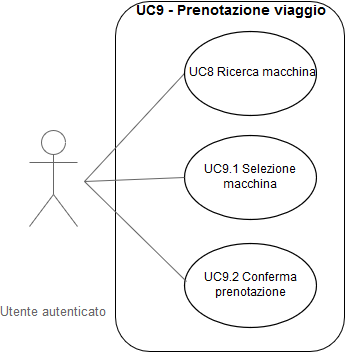
\includegraphics[scale=0.60]{immagini/9.png}    
           \caption{Diagramma UC9 - Prenotazione viaggio}
           \end{center}
            \end{figure}  
                  
            
       
     
       \subsubsection{UC 10-Recensione esperienza viaggio}
       \begin{itemize}
        \item \textbf{Attori primari}: Utente autenticato;
        \item \textbf{Attori secondari}: Aws;
        \item \textbf{Scopo e descrizione}: L'utente autenticato desidera recensire un viaggio che ha effettuato precedentemente.
        \item \textbf{Scenario principale}:
            \begin{itemize}
                \item L'utente ha effettuato l'accesso all'interno del sistema;
                \item L'utente a seguito di una ricerca ha scelto una macchina con la quale ha effettuato un viaggio;
                \item L'utente ha terminato il suo viaggio e visualizza una schermata in cui è possibile lasciare una recensione sul viaggio appena effettuato.
            \end{itemize}
        
        \item \textbf{Scenario secondario}: L'utente non desidera procedere con la recensione: la recensione non viene memorizzata dal sistema.
       
        
        \item \textbf{Precondizione}: L'utente è autenticato all'interno del sistema ed ha effettuato e concluso un viaggio. L'utente è quindi in grado di visualizzare una schermata in cui è in grado di recensire un viaggio che ha appena effettuato.
        \item \textbf{Postcondizione}: L'utente ha recensito l'esperienza di viaggio che ha concluso, ottenendo i premi previsti per la gamification all'interno dell'app.
        \end{itemize}  
      
      
       \subsubsection{UC 11: Chiusura del viaggio}
  
        \begin{itemize}
        \item \textbf{Attori primari}: Utente autenticato;
        \item \textbf{Attori secondari}: Aws;
        \item \textbf{Scopo e descrizione}: L'utente che ha effettuato un viaggio conferma di voler chiudere; 
        \item \textbf{Scenario principale}:
            \begin{itemize}
                \item L'utente è autenticato all'interno della piattaforma;
                \item L'utente sta effettuando un viaggio
                \item L'utente desidera terminare il viaggio e quindi sceglie la funzionalità "Termina";
                \item L'utente conferma la terminazione del viaggio;
            \end{itemize}
         
        \item \textbf{Inclusioni}:
             \begin{itemize}
                \item L'utente conferma la conclusione del viaggio (UC 11.1);
            \end{itemize}
        \item \textbf{Precondizione}: L'utente è riconosciuto nel sistema e sta effettuando correntemente un viaggio previa prenotazione;
        \item \textbf{Postcondizione}: L'utente conclude il viaggio e visualizza una schermata riassuntiva con possibilità di recensire.
        \end{itemize}


        \paragraph{UC 11.1:Conferma chiusura viaggio}
            \begin{itemize}
                \item \textbf{Attori primari}: Utente autenticato;
                
                \item \textbf{Scopo e descrizione}: L'utente conferma di voler effettuare la terminazione del viaggio che sta effettuando; 
                \item \textbf{Scenario principale}:
                    \begin{itemize}
                        \item L'utente si trova nella dashboard dedicata ai dati relativi al viaggio;
                        \item L'utente conferma l'operazione di terminazione del viaggio cliccando il pulsante apposito.
                    \end{itemize}
                \item \textbf{Precondizione}:L'utente si trova in una schermata in cui è possibile dare la conferma
                del termine del viaggio;
                \item \textbf{Postcondizione}:L’utente ha espresso di voler procedere con la terminazione del viaggio e quindi la procedura si conclude.
            \end{itemize}
        

        
            
       \subsubsection{UC 12-Visualizzazione dati personali relativi all'utente}  
      \begin{itemize}
        \item \textbf{Attori primari}: Utente autenticato;
        \item \textbf{Attori secondari}: Aws;
        \item \textbf{Scopo e descrizione}: L'utente visualizza i dati personali come nome, cognome, mail, username, dati opzionali e recensioni relativi al proprio account; 
        \item \textbf{Scenario principale}: L'utente autenticato richiede al sistema di visualizzare i propri dati personali;
        \item \textbf{Precondizione}: L'utente autenticato si trova nella propria area personale;
        \item \textbf{Postcondizione}: L'utente autenticato ottiene la visualizzazione dei dati personali.
        \end{itemize}  
        
     
        
      \subsubsection{UC 13-Visualizzazione dati relativi alle macchine messe a disposizione dall'utente}
        \begin{itemize}
        \item \textbf{Attori primari}: Utente autenticato;
        \item \textbf{Attori secondari}: Aws;
        \item \textbf{Scopo e descrizione}: L'utente visualizza una lista con le auto messe a disposizione da lui, visualizzando per ogni auto le varie caratteristiche; 
        \item \textbf{Scenario principale}: L'utente richiede al sistema di visualizzare le proprie auto;
        \item \textbf{Precondizione}: L'utente si trova nella propria area personale;
        \item \textbf{Postcondizione}: L'utente visualizza una lista con le sue auto messe a disposizione.
        \end{itemize}
 
            
         \subsubsection{UC 14-Visualizzazione itinerari compiuti dall'utente}
        \begin{itemize}
        \item \textbf{Attori primari}: Utente autenticato;
        \item \textbf{Attori secondari}: Aws;
        \item \textbf{Scopo e descrizione}: L'utente visualizza una lista con i viaggi compiuti, visualizzando per ogni viaggio, luogo di partenza, orario di partenza, luogo di arrivo, orario di arrivo, distanza percorsa, fattura; 
        \item \textbf{Scenario principale}: L'utente richiede al sistema di visualizzare gli itinerari compiuti;
        \item \textbf{Precondizione}: L'utente si trova nella propria area personale;
        \item \textbf{Postcondizione}: L'utente visualizza una lista con gli itinerari compiuti, o se in mancanza di tali mostrerà una schermata vuota.
        \end{itemize}    
            
 
        \subsubsection{UC 15-Visualizzazione del profilo di un altro utente}
        \begin{itemize}
            \item  \textbf{Attori primari}: Utente autenticato;
            \item \textbf{Attori secondari}: Aws;
            \item \textbf{Scopo e descrizione}: L'utente desidera avere più informazioni su un utente.
            \item \textbf{Scenario principale}: L'utente visualizza il profilo di un altro utente.
            \item \textbf{Precondizione}: L'utente è autenticato;
            \item \textbf{Postcondizione}: Il sistema ha elaborato la richiesta e presenta una schermata contenente le informazioni dell'utente
        \end{itemize}   
  
        
        
    \subsubsection{UC 16-Visualizzazione statistiche personali}  
      \begin{itemize}
        \item \textbf{Attori primari}: Utente autenticato;
        \item \textbf{Attori secondari}: Aws;
        \item \textbf{Scopo e descrizione}: L'utente visualizza i dati personali relativi alle proprie statistiche relative al suo utilizzo dell'applicazione. I dati visualizzabili in questa sezione precisamente sono:
            \begin{itemize}
                \item Stato di avanzamento dell'utente in termini di punti rank e badge;
                \item Visualizzazione statistiche azioni fatte all'interno dell'applicazione: numero viaggi, numero prenotazioni, km medi effettuati per viaggio;
                \item Missioni conclusioni, da fare, visualizzare missioni giornaliere sbloccate;
                \item Visualizzazione badge ottenuti.
            \end{itemize}
        \item \textbf{Scenario principale}: L'utente autenticato richiede al sistema di visualizzare i propri dati personali relativi alle statistiche di utilizzo dell'applicazione;
        \item \textbf{Precondizione}: L'utente autenticato si trova nella propria area personale;
        \item \textbf{Postcondizione}: L'utente autenticato ottiene la visualizzazione dei dati personali relativi alle statistiche di utilizzo dell'applicazione.
        \end{itemize}  
  
    \subsubsection{UC 17-Visualizzazione classifiche generali}  
      \begin{itemize}
        \item \textbf{Attori primari}: Utente autenticato;
        \item \textbf{Attori secondari}: Aws;
        \item \textbf{Scopo e descrizione}: L'utente visualizza i dati personali relativi alle classifiche generali calcolate dalla piattaforma. Le classifiche in questa sezione precisamente sono:
            \begin{itemize}
                \item Classifica globale assoluta sulla base dei punti rank degli utenti della piattaforma. La classifica è calcolata su scala decrescente: tanti più punti un utente possiede tanto più alta sarà la sua posizione;
                \item Classifica globale mensile sulla base dei punti rank degli utenti della piattaforma. Il posizionamento degli utenti è calcolato nello stesso modo della scala assoluta, solamente che vengono conteggiati esclusivamente i punti acquisiti su base mensile, non assoluta.
            \end{itemize}
            
        \item \textbf{Scenario principale}: L'utente autenticato richiede al sistema di visualizzare i dati personali relativi alle classifiche interne all'applicazione;
        \item \textbf{Precondizione}: L'utente è autenticato nel sistema;
        \item \textbf{Postcondizione}: L'utente autenticato ottiene la visualizzazione delle classifiche interne all'applicazione.
        \end{itemize}  
     
         
        
        
    \subsubsection{UC 18-Visualizzazione buoni spesa personali}  
      \begin{itemize}
        \item \textbf{Attori primari}: Utente autenticato;
        \item \textbf{Attori secondari}: Aws;
        \item \textbf{Scopo e descrizione}: L'utente visualizza i dati personali relativi ai buoni spesa (ovvero buoni sconto utilizzabili in aziende partner alla piattaforma) ottenuti/ottenibili/da riscuotere/riscossi dall'utente.
        \item \textbf{Scenario principale}: L'utente autenticato richiede al sistema di visualizzare i buoni spesa relativi all'utente;
        \item \textbf{Precondizione}: L'utente è autenticato nel sistema;
        \item \textbf{Postcondizione}: L'utente autenticato ottiene la visualizzazione dei buoni sconto che la piattaforma offre.
        \end{itemize}
  
    
            
    \subsubsection{UC 19-Riscuoti buono}  
      \begin{itemize}
        \item \textbf{Attori primari}: Utente autenticato;
        \item \textbf{Attori secondari}: Aws;
        \item \textbf{Scopo e descrizione}: L'utente intende utilizzare il buono sconto da lui cumulato presso aziende partner alla piattaforma. Con l'azione di riscossione notifica la sistema che ha utilizzato il buono disponibile, pertanto tale buono non è più utilizzabile in futuro.
        \item \textbf{Scenario principale}:
            \begin{itemize}
                \item L'utente autenticato si trova nella sezione di visualizzazione da buoni da lui cumulati;
                \item L'utente seleziona un buono tra quelli che ha cumulato;
                \item L'utente l'utente esprime la volontà di utilizzare il buono utilizzato
                
            \end{itemize}
            
        \item \textbf{Scenario secondario}: L'utente non intende proseguire con l'utilizzo del buono, l'azione non viene memorizzata nel sistema
         \item \textbf{Inclusioni}:
            \begin{itemize}
                \item L'utente seleziona il buono da utilizzare (UC 19.1);
                \item L'utente conferma di voler usufruire del buono da lui disposto(UC 19.2).
            \end{itemize}
          
        \item \textbf{Precondizione}: L'utente è autenticato nel sistema, si trova nella sezione di visualizzazione dei buoni e ha a disposizione almeno un buono da utilizzare;
        \item \textbf{Postcondizione}: L'utente autenticato usufruisce del buono spesa da lui posseduto.
        \end{itemize}  
        
            
    \subparagraph{UC 19.1-Selezione buono di cui usufruire}
    \begin{itemize}
                \item \textbf{Attori primari}: Utente autenticato;
                
                 \item \textbf{Scopo e descrizione}: L’utente seleziona uno tra i buoni a lui a disposizione per poterne usufruire;
                 \item \textbf{Scenario principale}: 
                 \begin{itemize}
                     \item L’utente si trova nella sezione dedicata alla visualizzazione dei buoni disponibili;
                     \item L'utente seleziona uno tra i buoni disponibili del quale vuole usufruire.          \end{itemize}
                 \item \textbf{Precondizione}: L’utente si trova in una schermata in cui è possibile selezionare il buono su cui si vuole riscuotere uno sconto;
                 \item \textbf{Postcondizione}: L’utente seleziona il buono che intende utilizzare.
                 \end{itemize}
    
    \subparagraph{UC 19.2-Conferma riscossione buono}
    \begin{itemize}
                \item \textbf{Attori primari}: Utente autenticato;
               
                 \item \textbf{Scopo e descrizione}: L’utente conferma di voler riscuotere il buono sconto precedentemente utilizzato per permettere al sistema di memorizzare la scelta;
                 \item \textbf{Scenario principale}: 
                 \begin{itemize}
                     \item L’utente si trova nella sezione dedicata alla riscossione dei buoni a lui disponibili;
                     \item L'utente conferma l'operazione di riscossione del buono cliccando il pulsante apposito. 
                 \end{itemize}
                 \item \textbf{Precondizione}: L’utente si trova in una schermata in cui è possibile dare la conferma dell'operazione di riscossione;
                 \item \textbf{Postcondizione}: L’utente ha espresso di voler procedere con la riscossione del buono.
                 \end{itemize}
                   
    \begin{figure}[h!]
           \begin{center}
           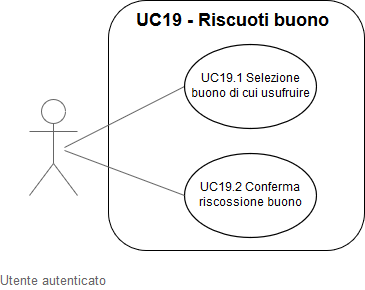
\includegraphics[scale=0.50]{immagini/19.png}    
           \caption{Diagramma UC19 - Riscuoti buono}
           \end{center}
            \end{figure}  
   
     
               
       \subsubsection{UC 20-Visualizzazione sezione esplora}  
      \begin{itemize}
        \item \textbf{Attori primari}: Utente autenticato;
        \item \textbf{Attori secondari}: Aws;
        \item \textbf{Scopo e descrizione}: L'utente visualizza i dati relativi alla sezione "esplora", all'interno della quale l'utente può visualizzare offerte relative alla zona in cui risiede, quali promozioni temporanee in partnership con aziende.
            
        \item \textbf{Scenario principale}: L'utente autenticato richiede al sistema di visualizzare la sezione dell'applicazione "esplora";
        \item \textbf{Precondizione}: L'utente è autenticato nel sistema;
        \item \textbf{Postcondizione}: L'utente autenticato ottiene la visualizzazione della sezione esplora.
        \end{itemize}        
     
                 
        \subsubsection{UC 21-Visualizzazione ruota dei premi}  
      \begin{itemize}
        \item \textbf{Attori primari}: Utente autenticato;
        \item \textbf{Attori secondari}: Aws;
        \item \textbf{Scopo e descrizione}: L'utente che visualizza la ruota della fortuna ha la possibilità di ricevere dei premi quando si ferma.
           
            
        \item \textbf{Scenario principale}: L'utente autenticato accede per la prima volta nella giornata nell'applicazione, visualizza la ruota della fortuna che consente di ricevere premi all'interno dell'applicazione, la ferma ed eventualmente riceve un premio;
        \item \textbf{Precondizione}: L'utente è autenticato nel sistema;
        \item \textbf{Postcondizione}: L'utente autenticato ottiene la visualizzazione della ruota della fortuna.
        \end{itemize}  
      
 
    
        
         
    
        
        
           
        
        
       

    
    
                \newpage
            \section{Requisiti}
                Di seguito vengono riportati tutti i requisiti individuati. Essi derivano dai casi d’uso,
dal capitolato, dagli incontri con il proponente oppure da necessità interne. Per essere
più leggibili verranno separati in tabelle a seconda della loro categoria. Di ogni requisito
verranno indicati: tipologia, priorità e provenienza.
I requisiti dovranno essere classificati per tipo e importanza utilizzando la sintassi definita nel documento \NdP.
\subsection{Classificazione dei requisiti} 
    \subsubsection{Requisiti funzionali}
    Definizione requisiti delle funzioni/caratteristiche che deve fare/avere il sistema
    
%\begin{longtable}[H]

    \taburowcolors[2] 2{tableLineOne .. tableLineTwo}
    \tabulinesep = 15pt
    \everyrow{\tabucline[.4mm  white]{}}
    
    \begin{longtabu} to \textwidth { X[l] X[l] X[l] }
        \tableHeaderStyle
        Identificatore & Descrizione & Fonti \\
        
         %REGISTRAZIONE, DA RCF001 A RCF025
         RCF001 &  Un utente può creare un account per usufruire delle funzionalità offerte & UC 2, Capitolato \\
         
         RCF002 &  La registrazione per essere effettuata richiede l'inserimento del nome da associare all'account &  UC 2.1, Verbale 2019.03.12 \\
         
         RCF003 &  La registrazione per essere effettuata richiede l'inserimento del cognome da associare all'account  &  UC 2.2, Verbale 2019.03.12 \\
         
         RCF004 &  La registrazione per essere effettuata richiede l'inserimento della mail da associare all'account  &  UC 2.3, Verbale 2019.03.12 \\
         
         RCF005 &  La registrazione per essere effettuata richiede l'inserimento della password da associare all'account  &  UC 2.4, Verbale 2019.03.12 \\
         
         RCF006 &  La registrazione per essere effettuata richiede la conferma della password precedentemente inserita da associare all'account  &  UC 2.5, Verbale 2019.03.12 \\
         
         
         RCF007 &  La registrazione per essere effettuata richiede l'inserimento dell'username da associare all'account  &  UC 2.6, Verbale 2019.03.12 \\
         
         RCF008 &  La registrazione per essere effettuata deve essere confermata &  UC 2.7 \\
         
         
         RCF009 &  Il sistema segnala errore nel caso in cui la password inserita nel campo "ridigita password" sia diversa da quella inserita nella prima digitazione &  UC 2.8 \\
         
         
         RCF010 &  Il sistema segnala errore nel caso in cui la mail fornita per la registrazione sia associata già a un altro account sulla piattaforma &  UC 2.9, Interno \\
         
          
         RCF011 &  Il sistema segnala errore nel caso in cui l'username fornito per la registrazione sia associato già a un altro account sulla piattaforma  &  UC 2.10, Interno \\
         
         
         RCF012 &  Il sistema segnala errore nel caso in cui la password fornita per la registrazione non sia nel formato corretto
         &  UC 2.11, Interno \\
         
         
         
         RCF0013 &  Il sistema segnala errore nel caso in cui la mail fornita per la registrazione non sia nel formato corretto
         &  UC 2.12, Interno \\
         
         
         RCF014 &  Il sistema segnala errore nel caso in cui la registrazione tenti di essere inviata non avendo tutti i campi compilati &  UC 2.13, Interno \\
         
         
         RDF015 &  Una volta effettuata la registrazione il sistema assegna all'utente 0 punti spesa & Interno \\
         
         
         RDF016 &  Una volta effettuata la registrazione il sistema assegna all'utente il badge "Principiante" & Interno \\
         
         
         RCF017 &  Una volta effettuata la registrazione l'utente all'interno del proprio profilo non ha associata alcuna vettura & Interno \\
         
         
         RCF018 &  Una volta effettuata la registrazione l'utente all'interno del proprio profilo non ha dati personali associati & Interno \\
         
         
          RCF019 &  Il sistema richiede un formato per la password ben preciso: deve essere di almeno sei caratteri, contenere almeno una lettera maiuscola e almeno un carattere speciale  & Interno \\
          
          
          RCF020 &  Il sistema richiede un formato per la mail ben preciso: caratteri alfa-numerici, seguiti dal carattere '@', seguito da un dominio & Interno \\
          
          
          RCF021 &  Il sistema richiede che un username all'interno della piattaforma sia unico. Non possono esistere due account con lo stesso username & Verbale 2019.03.25 \\
          
          
          RCF022 &  Il sistema richiede che la mail all'interno della piattaforma sia unica. Non possono esistere due account con la stessa mail & Verbale 2019.03.25 \\
           
           
          RCF023 &  Il sistema una volta eseguita l'operazione di registrazione assegna un unico nome, un unico cognome, un'unica password e un unico username per ogni account. Questo implica che, per esempio, un account non può avere associate due mail & Verbale 2019.03.25 \\
          
          
          RCF024 &  Il sistema una volta eseguita l'operazione di registrazione assegna zero punti al rank. & Interno \\
          
          
          RCF025 &  Il sistema una volta eseguita l'operazione di registrazione non assegna badge all'account appena creato. & Interno \\
         
         
         
         
         
         
         
         
         
         %LOGIN DA RCF026 A RCF034
         RCF026 &  Un utente dispone dell'operazione di login per accedere al proprio account all'interno della piattaforma &  UC 3, Capitolato \\
         
         
         RCF027 &  Il login per essere effettuato  richiede l'inserimento dell'username  associato al profilo a cui si vuole accedere &  UC 3.1 \\
          
          
         RCF028 &  Il login per essere effettuato  richiede l'inserimento della password  associata al profilo a cui si vuole accedere &  UC 3.2 \\
         
          
         RCF029 &  Il login per essere effettuato deve essere confermato &  UC 3.3 \\
         
         
         RCF030 &  Il sistema segnala errore nel caso in cui l'utente tenti di effettuare il login non avendo tutti i campi compilati &  UC 3.4, Interno \\
         
         
         RDF031 & Una volta effettuato il login l'utente viene indirizzato alla schermata principale &   Interno \\
           
         RCF032 &  Il login per essere effettuato deve contenere credenziali valide &  Interno \\
         
         
         RDF033 &  Il login effettuato per la prima volta fa ottenere punti rank all'utente &  Interno \\
         
         
         RDF034 &  Il login effettuato la prima volta in una giornata permette la visualizzazione di una ruota della fortuna che da la possibilità all'utente di ottenere bonus all'interno dell'applicazione &  Interno \\
         
         
         %LOGOUT: RCF035-RCF036
         RCF035 &  Un utente dispone dell'operazione di logout per uscire dal proprio account &  UC 4, Capitolato \\
         
         
         RDF036 &  Una volta eseguita correttamente l'operazione di logout l'utente viene reindirizzato dal sistema nella schermata principale &  Interno \\
         
         
         %GESTIONE DATI OPZIONALI DA RCF037 A RCF041
         RCF037 &  L'utente ha la possibilità di completare il proprio profilo (che in fase di creazione contiene solo dati obbligatori al fine della registrazione) con dati facoltativi supplementari, non richiesti in fase di registrazione. Tali informazioni sono: età, sesso, città di residenza, numero della patente, data di rilascio della patente, occupazione, collegamento al profilo facebook personale &  UC 5, Interno \\
         
         
         RCF038 &  I dati facoltativi possono essere aggiunti o aggiornati all'interno del profilo utente in qualsiasi momento &  Interno \\
         
         
         RDF039 & Il primo inserimento di dati facoltativi supplementari assegna punti bonus all'utente &  Interno \\
         
         
         RCF040 & I dati opzionali con cui un utente può completare il profilo sono: foto, sesso, età, città, collegamento con social facebook &  Interno \\
         
         
         RDF041 & Il collegamento all'account facebook fa ottenere all'utente particolari bonus all'interno della piattaforma &  Interno \\
              
            
         %GESTIONE DATI PERSONALI, DA RCF042 A RCF056 
         RCF042 & L'utente ha la possibilità di modificare alcuni dei campi obbligatori associati al proprio profilo &  UC 6, Verbale 2019.03.12 \\
         
         
         RCF043 & L'utente ha la possibilità di aggiornare la password associata al proprio profilo &  UC 6.1, Verbale 2019.03.12 \\
         
         
         RCF044 & Per aggiornare la password associata al profilo dell'utente il sistema richiede, a scopi di sicurezza, di inserire la vecchia password &  UC 6.1.1, Verbale 2019.03.12 \\
         
         
         RCF045 & Per aggiornare la password associata al profilo dell'utente il sistema richiede di inserire la nuova password due volte &  UC 2.5 \\
         
         
         RCF046 & Il sistema segnala un errore nel caso in cui l'utente tenti di aggiornare la password associata al profilo con una password uguale a quella già salvata all'interno del profilo &  UC 6.1.2, Verbale 2019.03.12 \\
         
         
         RCF047 & Il sistema segnala un errore nel caso in cui l'utente tenti di aggiornare la password associata al profilo inserendo nel campo di "Ripeti password" una password diversa da quella della prima digitazione &  UC 2.8 \\
         
         
         RCF048 & Il sistema segnala un errore nel caso in cui l'utente tenti di aggiornare la password associata al profilo inserendo una password che non rispetti il formato richiesto (precedentemente espresso) &  UC 2.11 \\
           
         
         RCF049 & L'utente ha la possibilità di aggiornare la mail associata al proprio profilo & UC 6.2, Verbale 2019.03.12 \\
         
         
         RCF050 & Il sistema segnala un errore nel caso in cui l'utente tenti di aggiornare la mail associata al profilo inserendo una mail già associata ad un altro profilo presente nella piattaforma &  UC 2.9, Verbale 2019.03.12\\
         
         
          
         RCF051 & L'utente ha la possibilità di aggiornare il nome associato al proprio profilo & UC 6.3, Verbale 2019.03.12 \\
         
         
         RCF052 & L'utente ha la possibilità di aggiornare il cognome associato al proprio profilo & UC 6.4, Verbale 2019.03.12 \\
         
         
         RCF053 & L'utente ha la possibilità di eliminare il proprio profilo & UC 6.5, Verbale 2019.03.12 \\
         
         
         RCF054 & L'utente deve confermare la modifica per effettuare l'aggiornamento sui dati & UC 6.6 \\
         
         
         RCF055 & L'utente ha la possibilità di effettuare l'aggiornamento dei propri dati obbligatori all'interno del profilo in qualsiasi momento & Verbale 2019.03.12  \\
         
         
         RDF056 & Nel caso l'utente cambi idea durante l'operazione di modifica e voglia ripristinare i dati precedenti, il sistema permette di annullare le modifiche tenendo in memoria gli ultimi dati relativi al profilo dell'utente & Verbale 2019.03.12  \\
         
         
         %GESTIONE DELLE MACCHINE DEL PROFILO UTENTE, da RCF057 A RCF098
         
         RCF057 & L'utente ha la possibilità di gestire (ovvero aggiungere, modificare o eliminare) le macchine e relativi dati associati al proprio profilo &  UC 7, Capitolato \\
         
         
         RCF058 & L'utente in particolare ha la possibilità di aggiungere auto da associare al proprio profilo. Le auto inserite all'interno di un profilo indicano le vetture che l'utente rende disponibili agli altri utenti per effettuare dei viaggi con esse &  UC 7.1, Capitolato \\
         
         
         RCF059 & L'aggiunta di una nuova auto da associare al profilo utente richiede l'inserimento della targa della stessa &  UC 7.1.1, Verbale 2019.03.25 \\
         
         
         RCF060 & L'aggiunta di una nuova auto da associare al profilo utente richiede l'inserimento della marca della stessa &  UC 7.1.2, Verbale 2019.03.25 \\
          
          
          RCF061 & L'aggiunta di una nuova auto da associare al profilo utente richiede l'inserimento del modello della stessa &  UC 7.1.3, Verbale 2019.03.25 \\
          
          
          RCF062 & L'aggiunta di una nuova auto da associare al profilo utente richiede l'inserimento dell'anno di produzione della stessa &  UC 7.1.4, Verbale 2019.03.25 \\
          
          
          RCF063 & L'aggiunta di una nuova auto da associare al profilo utente richiede l'inserimento dei cavalli motore della stessa &  UC 7.1.5, Verbale 2019.03.25 \\
          
          
          RCF064 & L'aggiunta di una nuova auto da associare al profilo utente richiede l'inserimento della cilindrata della stessa & UC 7.1.6, Verbale 2019.03.25 \\
          
          
          RCF065 & L'aggiunta di una nuova auto da associare al profilo utente richiede l'inserimento del raggio di percorrenza consentito per la stessa. Con raggio di percorrenza s'intende il numero di km che il proprietario concede di effettuare per un viaggio con la sua vettura. Nel caso in cui il proprietario non voglia porre alcun limite tale valore viene settato a infinito & UC 7.1.7, Verbale 2019.03.25 \\
          
          
          RCF066 & L'aggiunta di una nuova auto da associare al profilo utente richiede l'inserimento del chilometraggio della stessa & UC 7.1.8, Verbale 2019.03.25 \\
          
          
          RCF067 & L'aggiunta di una nuova auto da associare al profilo utente richiede l'inserimento di un calendario di disponibilità della stessa, che specifica in che giorni l'utente mette a disposizione l'auto per gli altri utenti & UC 7.1.9\\
          
          
          RCF068 & L'aggiunta di una nuova auto da associare al profilo utente richiede l'inserimento di una tariffa oraria per la stessa & UC 7.1.10\\
          
          
          RCF069 & Il sistema segnala errore nel caso in cui un utente tenti di inserire una nuova vettura lasciando almeno uno dei campi sopracitati (targa, modello, marca, anno, cavalli, cilindrata, raggio e chilometraggio) vuoti & UC 7.1.11, Verbale 2019.03.25 \\
          
          
          RCF070 & Il sistema segnala errore nel caso in cui un utente tenti di inserire una nuova vettura compilando il campo targa con dati non nel formato corretto. Il formato richiesto per una targa sono caratteri alfanumerici e un numero di caratteri minimi uguale a 6 & UC 7.1.12, Verbale 2019.03.25 \\
          
          
          RCF071 & Il sistema segnala errore nel caso in cui un utente tenti di inserire una nuova vettura con un numero di targa uguale a quello già associato ad un altro profilo & UC 7.1.13, Verbale 2019.03.25 \\
          
          
          RCF072 & Il sistema segnala errore nel caso in cui un utente tenti di inserire una nuova vettura compilando in modo errato (ovvero con valori numerici minori di zero) almeno uno dei seguenti campi: anno, cavalli, cilindrata, raggio, chilometraggio & UC 7.1.14 \\
          
          
          RCF073 & L'utente una volta inserita un'auto associata al suo profilo successivamente ha la possibilità di modificarne i dati. &  UC 7.2, Verbale 2019.03.25 \\
          
          
          RCF074 & Per effettuare l'operazione di modifica dell'auto il sistema richiede prima di selezionare l'auto della quale si intendono modificare i dati &  UC 7.2.1,  \\
          
          
          RCF075 & Per effettuare l'operazione di modifica dell'auto il sistema richiede la conferma della modifica &  UC 7.2.2,  \\
          
          
          RCF076 & Il sistema permette di modificare la targa di una macchina precedentemente inserita nell'account &  UC 7.2.3, Verbale 2019.03.25 \\
          
          
          RCF077 & Il sistema permette di modificare la marca di una macchina precedentemente inserita nell'account &  UC 7.2.4, Verbale 2019.03.25 \\
          
          
          RCF078 & Il sistema permette di modificare il modello di una macchina precedentemente inserita nell'account &  UC 7.2.5, Verbale 2019.03.25 \\
          
          
          RCF079 & Il sistema permette di modificare l'anno di produzione di una macchina precedentemente inserita nell'account &  UC 7.2.6, Verbale 2019.03.25 \\
          
          
          RCF080 & Il sistema permette di modificare i cavalli motore di una macchina precedentemente inserita nell'account &  UC 7.2.7, Verbale 2019.03.25 \\
          
          
          RCF081 & Il sistema permette di modificare  la cilindrata del motore di una macchina precedentemente inserita nell'account &  UC 7.2.8, Verbale 2019.03.25 \\
          
          
          RCF082 & Il sistema permette di modificare il raggio di percorrenza consentito di una macchina precedentemente inserita nell'account &  UC 7.2.9, Verbale 2019.03.25 \\
          
          
         RCF083 & Il sistema permette di modificare il chilometraggio di una macchina precedentemente inserita nell'account &  UC 7.2.10, Verbale 2019.03.25 \\
         
         RCF084 & Il sistema permette di modificare il calendario di disponibilità di una macchina precedentemente inserita nell'account &  UC 7.2.11, Verbale 2019.03.25 \\
         
         
         RCF085 & Il sistema permette di modificare la tariffa oraria di una macchina precedentemente inserita nell'account &  UC 7.2.12, Verbale 2019.03.25 \\
         
         
         RCF086 & Il sistema segnala errore nel caso in cui l'utente tenti di modificare la targa di una vettura con un numero di targa in un formato non consentito  &  UC 7.1.12, Verbale 2019.03.25 \\
         
         
         RCF087 & Il sistema segnala errore nel caso in cui l'utente tenti di modificare la targa di una vettura con un numero di targa già esistente all'interno della piattaforma  &  UC 7.1.13, Verbale 2019.03.25 \\
         
         
         RCF088 & Il sistema segnala errore nel caso in cui l'utente tenti di modificare uno o più tra i campi anno, cilindrata, cavalli, raggio o chilometraggio con dati numerici minori di zero  &  UC 7.1.14, Verbale 2019.03.25 \\
         
         
         RCF089 & L'utente  ha la possibilità di eliminare un'auto precedentemente aggiunta all'interno del proprio profilo. Eliminando l'auto dall'account l'utente esprime la volontà che essa non possa più venire utilizzata per effettuare viaggi da parte di altri utenti &  UC 7.3, Verbale 2019.03.25 \\
         
         
         RCF090 & Il sistema permette ad ogni utente in possesso di un account di associare una o più autovettore per il proprio profilo &   Verbale 2019.03.25 \\
         
         
         RCF091 & Il sistema permette di associare esclusivamente autovetture all'interno di un profilo. Questo significa che mezzi come camion, camper, roulotte non sono consentiti  &   Verbale 2019.03.25 \\
         
         
         RCF092 & Il sistema assegna un bonus in termini di punti ad un utente che inserisce la sua prima autovettura all'interno del profilo &   Verbale 2019.03.25 \\
         
         
         RCF093 & Il sistema non permette all'utente di effettuare la modifica dei dati relativi ad un'auto se nel frattempo un altro utente sta effettuando un viaggio con quella vettura. L'utente che desidera effettuare la modifica dovrà attendere il termine del viaggio &   Verbale 2019.03.25 \\
         
         
         RCF094 & Il sistema permette all'utente di effettuare una modifica su un'auto da lui precedentemente associata al profilo in qualsiasi momento &   Verbale 2019.03.25 \\
         
         
         RCF095 & Il sistema permette all'utente di modificare i dati relativi a un auto solo se è stata precedentemente inserita almeno un auto &   Verbale 2019.03.25 \\
         
         
         RDF096 & Il primo inserimento di un auto attribuisce bonus all'utente &   Interno \\
         
         
         RDF097 & Il sistema attribuisce bonus all'utente che inserisce una tariffa oraria minore alla media per una delle sue auto &   Interno \\
         
         
         RDF098 & Il sistema permette all'utente di stabilire un calendario di disponibilità con ripetizione settimanale &   Interno \\
         
         
         %RICERCA AUTO, DA RCF099 A RC107
         RCF099 &  Un utente può effettuare una ricerca per visualizzare le auto che la piattaforma mette a disposizione per effettuare un viaggio & UC 8, Capitolato \\
         
         
         RCF100 &  Per effettuare una ricerca l'utente deve inserire le zone (partenza e arrivo) all'interno delle quali vuole effettuare il viaggio & UC 8.1, Capitolato \\
         
         
         RCF101 &  Per effettuare una ricerca l'utente deve inserire i giorni con l'orario (partenza e arrivo) all'interno dei quali vuole effettuare il viaggio & UC 8.2, Capitolato \\
         
         
         RCF102 &  Per effettuare una ricerca l'utente deve inserire il prezzo massimo che desidera pagare per effettuare il viaggio & UC 8.3, Capitolato \\
         
         
         RCF103 &  Per effettuare una ricerca l'utente deve inserire le caratteristiche che desidera per l'auto con cui effettuare il viaggio & UC 8.4, Interno \\
         
         
         RCF104 &  Per effettuare l'operazione di ricerca il sistema richiede la conferma da parte dell'utente  & UC 8.5, Interno \\
         
         
         RCF105 &  Il sistema segnala errore nel caso in cui l'utente tenti di eseguire una ricerca compilando i campi richiesti con un formato sbagliato & UC 8.6, Interno \\
         
         
         RCF106 &  Il sistema permette ad un utente loggato di eseguire una ricerca in qualsiasi momento & Interno \\
         
         
         RDF107 &  Il sistema visualizza i risultati di una ricerca in ordine di migliore corrispondenza & Interno \\
         
         
         %PRENOTAZIONE DA RCF0108 A RCF118
         RCF108 &  Un utente può prenotare un'auto con la quale effettuare un viaggio & UC 9, Capitolato \\
         
         
         RCF109 &  La prenotazione è effettivamente memorizzata nel sistema nel momento in cui il proprietario dell'auto conferma la prenotazione & Interno \\
         
         RDF110 &  La prenotazione non può essere effettuata se l'utente ha un viaggio in corso & Interno \\
         
         
         RDF111 &  La prenotazione può essere annullata fino a dodici ore prima dell'inizio del viaggio & Interno \\
         
         
         RCF112 &  Il sistema assegna dei bonus all'utente che effettua la prima prenotazione   & Interno \\
         
         
         RDF113 &  Il sistema permette prenotazioni di viaggi che durano più di ventiquattro ore & Interno \\
         
         
         RCF114 & Quando un utente richiede la prenotazione di un auto, il sistema notifica al proprietario di tale richiesta, presentandogli una schermata che gli permette di accettare, rifiutare o contattare l'utente che ha effettuato la richiesta & Interno \\
         
         
         RCF115 & Quando una prenotazione viene effettuata il sistema notifica al proprietario dell'auto l'avvenuta prenotazione   & Interno \\
         
         
         RDF116 &  Il sistema assegna un bonus all'utente proprietario che da in prestito l'auto ad un utente con rank basso & Interno \\
         
         
         RDF117 &  Il sistema assegna un bonus all'utente proprietario dopo un certo numero di prestiti & Interno \\
         
         
         RDF118 &  Il sistema assegna un bonus all'utente proprietario che presta auto agli utenti che desiderano percorrere lunghe tratte (maggiori di cento chilometri) & Interno \\
         
         
         %RECENSIONE VIAGGIO da rcf 119 a rcf 122
         RCF119 &  Un utente, a seguito della conclusione di un viaggio, può recensire il viaggio effettuato & UC 10, Verbale 2019.03.12 \\
         
         
         RCF120 &  Un utente può recensire il viaggio da lui effettuato dal momento in cui conclude il viaggio fino ad un massimo di quarantotto ore dopo & Interno \\
         
         
         RDF121 &  Il sistema assegna il bonus all'utente quando egli raggiunge una certa soglia di recensioni (la prima, dopo cinque, dopo venticinque, dopo cinquanta, dopo cento e dopo cinquecento) & Interno \\
         
         
         RDF122 &  Il sistema assegna il bonus all'utente quando egli raggiunge una certa soglia di recensioni positive da parte di altri utenti (la prima, dopo cinque, dopo venticinque, dopo cinquanta, dopo cento e dopo cinquecento) & Interno \\
         
         
         %CHIUSURA VIAGGIO da rcf 123 a rcf 127
         RCF123 &  Un utente che sta eseguendo un viaggio, nel momento in cui arriva a destinazione può concludere il viaggio & UC 11, Capitolato \\
         
         
         RCF124 &  La chiusura del viaggio per essere eseguita richiede la conferma da parte dell'utente & UC 11.1, Interno \\
         
         
         RDF125 &  La chiusura di un viaggio può essere eseguita almeno dopo un minuto dall'inizio previsto del viaggio & Interno \\
         
         
         RDF126 &  La chiusura di un viaggio avviene automaticamente nel caso l'utente si dimentichi di eseguirla. La chiusura automatica avviene passate le quarantotto ore dall'orario di chiusura prevista  & Interno \\
         
         
         RDF127 &  Conclusa l'operazione di chiusura del viaggio sulla piattaforma, se l'utente ha collegato il proprio account facebook, il sistema permette di condividere l'esperienza di viaggio vissuta sul social  & Interno \\
         
         %VISUALIZZAZIONE DATI ANAGRAFICI PERSONALI da rcf 128
         RCF128 &  Un utente può visualizzare i propri dati personali all'interno del proprio profilo. Sono sempre visibili i dati anagrafici obbligatori richiesti in fase di registrazione e, opzionalmente se l'utente ha deciso di inserirli, i dati opzionali &  UC 12, Interno \\
         
        %VISUALIZZAZIONE statistiche PERSONALI da rcf 129, rcf130
        
         RCF129 &  Un utente può visualizzare le statistiche personali all'interno del proprio profilo. In particolare sono visualizzabili: lo stato di avanzamento del livello, le missioni fatte/da fare/sbloccate/giornaliere e le statistiche riguardanti i movimenti eseguiti dall'utente all'interno dell'applicazione &  UC 16, Interno \\
         
         
         %VISUALIZZAZIONE DATI macchine personali rcf130
         RCF130 &  Un utente può visualizzare i propri dati relativi alle macchine associate al proprio profilo &  UC 13, Interno \\
         
         
         %VISUALIZZAZIONE itinerari eseguiti personali rcf131, 
         RCF131 &  Un utente può visualizzare gli itinerari da lui eseguiti, ovvero visualizza un riepilogo di tutti i viaggi da lui effettuati prendendo in prestito un'auto dal profilo di un altro utente della piattaforma. In particolare sono visibili gli orari (partenza o arrivo), il tragitto percorso, il tempo impiegato per il viaggio e il prezzo speso per il viaggio &  UC 14, Interno \\
         
         
         %VISUALIZZAZIONE profilo altro utente da rcf132, rcf 134
         RCF132 &  Un utente può visualizzare il profilo di un qualsiasi utente registrato nella piattaforma &  UC 15, Interno \\
         
         
         RCF133 &  L'utente che visita il profilo di un altro utente è in grado di vederne i dati anagrafici obbligatori e, se esistono, i dati opzionali da lui inseriti &  UC 15, Interno \\
         
         
         RCF134 &  L'utente che visita il profilo di un altro utente è in grado di vederne i dati relativi alle sue statistiche: punti rank, badge conseguiti e statistiche dell'utente &  UC 15, Interno \\
         
         %VISUALIZZAZIONE CLASSIFICHE da rcf135 a rcf136
          RCF135 &  L'utente è in grado di visualizzare delle classifiche: una globale basata sui punti rank degli utenti, classifica basata sulle statistiche e su base mensile &  UC 17, Interno \\ 
          
          
          RDF136 & Un utente acquisisce punti bonus ogni qualvolta che compare primo in una delle classifiche della piattaforma presenti &   Interno \\ 
          
          
          %VISUALIZZAZIONE CLASSIFICHE da rcf137
          RCF137 &  L'utente è in grado di visualizzare i buoni promozionali associati al suo profilo: utilizzati, da utilizzare & UC 18\\ 
          
          
          
          %RISCUOTI BUONO rcf 138, 139, 140
          RCF138 &  L'utente è in grado di riscuotere i buoni da lui cumulati & UC 19\\ 
          
          
          RCF139 &  L'utente per riscuotere un determinato buono deve preventivamente selezionarlo & UC 19.1\\ 
          
          
          RCF140 &  L'utente per riscuotere un determinato buono deve confermare l'operazione & UC 19.2\\
          
          
          %ESPLORA
          RDF141 &  L'utente è in grado di visualizzare una sezione denominata "Esplora" all'interno della quale sono presenti promozioni a termine in partnership con aziende & UC 20\\ 
          
          
            
    \end{longtabu}

%\caption{Prospetto economico - Analisi}  
%\end{longtable}
    
    \newpage
    
    
    \subsubsection{Requisiti di qualità}
      \taburowcolors[2] 2{tableLineOne .. tableLineTwo}
    \tabulinesep = 15pt
    \everyrow{\tabucline[.4mm  white]{}}
    
    \begin{longtabu} to \textwidth { X[l] X[l] X[l] }
        \tableHeaderStyle
        Identificatore & Descrizione & Fonti \\
         RCQ001 &  Il materiale consegnato deve essere coerente con quello le norme definite nel documento \NdP e \PdQ  &  Interno \\
         
         RCQ002 &  Vengono forniti tutorial per l'uso dell'applicazione agli utenti  &  Interno \\
          
         RCQ003 & La progettazione rispetta tutte le norme e le metriche indicate nei documenti \NdP e \PdQ.  &  Interno \\
           
         RCQ004 & Il processo di sviluppo e manutenzione del software si avvale del processo di \citgl{Continuos Integration} &  Interno \\
         
         RCQ005 & Durante il processo di analisi e progettazione si deve tener conto delle problematiche di usabilità &  Interno \\
         
         RCQ006 & Durante il processo di analisi e progettazione si deve tener conto delle problematiche di user-experience &  Interno \\
         
         RCQ007 & L'interfaccia grafica deve essere intuitiva &  Interno \\
         
         
         
    \end{longtabu}
    
    \newpage
    
    \subsubsection{Requisiti di vincolo}
    \taburowcolors[2] 2{tableLineOne .. tableLineTwo}
    \tabulinesep = 15pt
    \everyrow{\tabucline[.4mm  white]{}}
    
    \begin{longtabu} to \textwidth { X[l] X[l] X[l] }
        \tableHeaderStyle
        Identificatore & Descrizione & Fonti \\
        
        RCV001 & Il sistema deve essere un'applicazione mobile composta da front-end (quasi totalmente fornito) e back-end.  &  Capitolato \\
        
        RDV002 & La parte di back-end è composta da una parte di interazione con servizi AWS (nello specifico la parte relativa al login) &  Verbale 2019.03.12 \\
        
        RCV003 & L'utente interagisce con un'applicazione in lingua italiana &  Capitolato \\
        
        RCV004 & L'applicazione deve includere meccanismi di \citgl{Gamification} &  Capitolato \\
        
        RCV005 & Per l'implementazione di meccanismi di Gamification viene fatto riferimento al modello \citgl{Octalysis} &  Capitolato \\
           
        RCV006 &  Per lo sviluppo dell'applicazione il linguaggio di programmazione utilizzato è Kotlin & Verbale 2019.03.12 \\
         
        RDV007 &  L'applicazione deve funzionare su piattaforma Android dalla versione 6 in poi & Verbale 2019.03.12 \\
          
        RCV008 &  L'IDE di riferimento per la creazione dell'app è \citgl{Android Studio} &  Verbale 2019.03.12  \\
        
        RDV009 & Il codice verrà reso disponibile open-source tramite repository online sulla piattaforma Github &  Verbale 2019.03.12  \\
          
        RDV010 & Devono essere eseguiti i \citgl{test UI} per tutti gli scenari dell'applicazione &  Verbale 2019.03.12 \\
           
        RDV011 & Come modello di sviluppo software viene indicato il modello "test-driven-development" (TDD) &  Verbale 2019.03.12 \\
           
        RDV012 & Viene utilizzato il framework Espresso per la creazione di test dell'interfaccia utente per simulare le interazioni di un utente con l'applicazione &  Verbale 2019.03.12 \\
           
           
           %tecnologie come angularjs da mettere come desiderabili anche se front end per lo più già fornito???
           
           
           
           
         
         
    \end{longtabu}
    
    
    
    \newpage


\subsection{Tracciamento}
    \subsubsection{Tracciamento fonti-requisiti}

    \taburowcolors[2] 2{tableLineOne .. tableLineTwo}
    \tabulinesep = 15pt
    \everyrow{\tabucline[.4mm  white]{}}
    %da rivedere
    
    \begin{longtabu} {X[c] X[c]}
    \hline
    Fonte & Requisiti individuati \\ 
     {Capitolato} &  RCF001, RCF026, RCF035, RCF057, RCF058, RCF099, RCF100, RCF101, RCF108, RCF123, RCV001, RCV003, RCV004, RCV005 \\ 
                                
                               
     {Interni} & RCF010, RCF011, RCF012, RCF013, RCF014, RCF015, RCF016, RCF017, RCF018, RCF019, RCF020,
     RCF024, RCF025,
     RCF030, RCF031, RCF032, RDF033, 
     RCF036, RCF037, RCF038, RCF039, RCF040, RDF041,
     RCF096, RCF097, RDF098,
     RCF102, RCF103, RCF104, RCF105, RCF106, RDF107,
     RCF109, RDF110, RDF111, RCF112, RDF113, RCF114, RCF115, RDF116, RDF117, RDF118,
     RCF120, RDF121, RDF122,
     RCF124, RDF125, RDF126, RDF127,
     RCF128, RCF130, RCF131, RCF132, RCF133, RCF134, RCF136, RCQ001, RCQ002, RCQ003, RCQ004, RCQ005, RCQ006, RCQ007 \\  
     
     
                             
    {Verbale 2019.03.12} & RCF002, RCF003, RCF004, RCF005, RCF006, RCF007, RCF041, RCF042, RCF043, RCF045, RCF048, RCF049, RCF050, RCF051, RCF052, RCF054, RCF055, RCF119, RDV002, RCV006, RDV007, RCV008, RDV009, RDV010, RDV011, RDV012 \\                   
    
   
   
   {Verbale 2019.03.25} & RCF021, RCF022, RCF023, RCF058, RCF059, RCF060, RCF061, RCF062, RCF063, RCF064, RCF065, RCF068, RCF069, RCF070, RCF071, RCF072, RCF075, RCF076, RCF077, RCF078, RCF079, RCF080, RCF081, RCF082, RCF085, RCF086, RCF087, RCF088, RCF089, RCF090, RCF091, RCF092, RCF093, RCF094 \\ 
   
   
   {UC 2} & RCF001 \\ 
   
   {UC 2.1} & RCF002 \\ 
   
   {UC 2.2} & RCF003 \\ 
   
   {UC 2.3} & RCF004 \\ 
   
   {UC 2.4} & RCF005 \\ 
   
   {UC 2.5} & RCF006, RCF045 \\
   
   {UC 2.6} & RCF007 \\ 
   
   {UC 2.7} & RCF008 \\ 
   
   {UC 2.8} & RCF009, RCF047 \\ 
   
   {UC 2.9} & RCF010, RCF050 \\
   
   {UC 2.10} & RCF011 \\ 
   
   {UC 2.11} & RCF012, RCF048 \\
   
   {UC 2.12} & RCF013 \\ 
   
   {UC 2.13} & RCF014 \\ 
   
   {UC 3} & RCF026 \\
   
   {UC 3.1} & RCF027 \\ 
   
   {UC 3.2} & RCF028 \\ 
   
   {UC 3.3} & RCF029 \\ 
   
   {UC 3.4} & RCF030 \\
   
   {UC 4} & RCF035 \\ 
   
   {UC 5} & RCF035 \\ 
   
   {UC 6} & RCF042 \\ 
   
   {UC 6.1} & RCF043 \\ 
   
   {UC 6.1.1} & RCF044 \\ 
   
   {UC 6.1.2} & RCF046 \\ 
   
   {UC 6.2} & RCF049 \\ 
   
   {UC 6.3} & RCF051 \\
   
   {UC 6.4} & RCF052 \\ 
   
   {UC 6.5} & RCF053 \\ 
   
   {UC 6.6} & RCF054 \\ 
   
   
   
   {UC 7} & RCF057 \\ 
   
   {UC 7.1} & RCF058 \\ 
   
   {UC 7.1.1} & RCF059 \\ 
   
   {UC 7.1.2} & RCF060 \\ 
   
   {UC 7.1.3} & RCF061 \\ 
   
   {UC 7.1.4} & RCF062 \\ 
   
   {UC 7.1.5} & RCF063 \\  
   
   {UC 7.1.6} & RCF064 \\ 
   
   {UC 7.1.7} & RCF065 \\ 
   
   {UC 7.1.8} & RCF066 \\  
   
   {UC 7.1.9} & RCF067 \\ 
   
   {UC 7.1.10} & RCF068 \\ 
   
   {UC 7.1.11} & RCF069 \\ 
   
   {UC 7.1.12} & RCF070, RCF086\\ 
   
   {UC 7.1.13} & RCF071, RCF087 \\ 
   
   {UC 7.1.14} & RCF072, RCF088 \\ 
   
   {UC 7.2} & RCF073 \\ 
   
   {UC 7.2.1} & RCF074 \\ 
   
   {UC 7.2.2} & RCF075 \\ 
   
   {UC 7.2.3} & RCF076 \\ 
   
   {UC 7.2.4} & RCF077 \\ 
   
   {UC 7.2.5} & RCF078 \\ 
   
   {UC 7.2.6} & RCF079 \\ 
   
   {UC7. 2.7} & RCF080 \\ 
   
   {UC 7.2.8} & RCF081 \\ 
   
   {UC 7.2.9} & RCF082 \\ 
   
   {UC 7.2.10} & RCF083 \\
   
   {UC 7.2.11} & RCF084 \\ 
   
   {UC 7.2.12} & RCF085 \\ 
 
    {UC 7.3} & RCF089 \\ 
    
    
    
   {UC 8} & RCF099 \\ 
   
   {UC 8.1} & RCF100 \\ 
   
   {UC 8.2} & RCF101 \\ 
   
   {UC 8.3} & RCF102 \\
   
   {UC 8.4} & RCF103 \\ 
   
   {UC 8.5} & RCF104 \\ 
   
   {UC 8.6} & RCF105 \\ 
   
   
   {UC 9} & RCF108 \\
   
   {UC 9.2} & RCF109 \\
   
   {UC 10} & RCF119 \\
   
   {UC 11} & RCF123 \\
   
   {UC 11.1} & RCF124 \\
   
   {UC 12} & RCF128 \\
   
   {UC 13} & RCF130 \\
   
   {UC 14} & RCF131 \\
   
   {UC 15} & RCF132 \\
   
   {UC 16} & RCF129 \\
   
   {UC 17} & RCF135 \\
   
   {UC 18} & RCF137 \\
   
   {UC 19} & RCF138 \\
   
   {UC 19.1} & RCF139 \\
   
   {UC 19.2} & RCF140 \\
   
    {UC 20} & RCF141 \\
    
    {UC 21} & RDF034 \\
                                
    
    \end{longtabu}
    
    
    
    
    
    
    
    
    
    
    
   
                \newpage
		    
		\newpage
\end{document}
